\begin{artengenv}{Jinyeong Gim}
	{The ontic-epistemic debates of explanation revisited: The three-dimensional approach}
	{The ontic-epistemic debates of explanation revisited$\ldots$}
	{The ontic-epistemic debates of explanation revisited: The three-di\-men\-sional approach}
	{Seoul National University, Republic of Korea}
	{After Wesley Salmon's causal-mechanical stance on explanation in the 1980s, the ontic-epistemic debate of scientific explanations appeared to be resolved in the philosophy of science. However, since the twenty-first century, this debate has been rekindled among philosophers who focus on mechanistic explanations. Nevertheless, its issues have evolved, necessitating scrutiny of the new trends in this debate and a~comparison with the original controversy between Carl Hempel and Salmon. The primary objective of this paper is to elucidate three categorical dimensions in the ontic-epistemic debates, spanning from the original to the recent controversies. Subsequently, it will explore why the conception of explanation is linked to representations, what conditions are necessary for linguistic expressions to be explanatory, and what roles norms play in explanation. Consequently, contrary to the common stereotype, it will be argued that mechanistic explanations are more likely to be epistemic rather than ontic.
	}
	{mechanistic explanation, scientific representation, explanatory norms, Wesley Salmon.}






\section*{Introduction}
\lettrine[loversize=0.13,lines=2,lraise=-0.03,nindent=0em,findent=0.2pt]%
{W}{}esley Salmon's initial distinction between the ontic and epistemic accounts of scientific explanation stood out as one of the most prominent differences between Hempel's and Salmon's perspectives
%\label{ref:RNDqFLZLus7w1}(Salmon, 1984; 1989).
\parencites*[][]{salmon_scientific_1984}[][]{salmon_four_1989}. %
 In broad terms, the epistemic account posits that scientific explanation involves an inferential argument aimed at understanding or predicting natural phenomena 
%\label{ref:RNDuL5cqHAJL9}(see Hempel and Oppenheim, 1948; Hempel, 1965).
\parencites[see][]{hempel_studies_1948}[][]{hempel_aspects_1965}. %
 On the other hand, the ontic account asserts that scientific explanation showcases the causal structures in the world that lead to the production of explanandum phenomena. Hempel's view faced numerous counterexamples, leading to the widespread acceptance of Salmon's perspective in the philosophy of science. Salmon's causal-mechanical explanation emerged as an alternative to Hempel's covering law model.\footnote{The original debate between the ontic and epistemic accounts of scientific explanation was not historically limited solely to Hempel and Salmon. Ellis 
%\label{ref:RNDcGdPGgloX4}(1956)
\parencite*[][]{ellis_relation_1956} %
 initiated this kind of controversy by focusing on the difference between explanation and description. Coffa 
%\label{ref:RNDbP9sjyGiJk}(1973)
\parencite*[][]{coffa_foundations_1973} %
 also engaged in criticizing Hempel's view 
%\label{ref:RNDEbFHqDafv3}(see Wright and van Eck, 2018).
\parencite[see][]{wright_ontic_2018}. %
 However, this paper concentrates on Salmon's criticisms of Hempel for the purpose of philosophical clarification.}

Mechanistic explanation serves as a~prototypical example of the ontic account of scientific explanation in line with Salmon's ideas. However, in the twenty-first century, some advocates of mechanistic explanation have posited that it is not ontic but rather epistemic
%\label{ref:RNDWRZPuTeL6v}(Bechtel and Abrahamsen, 2005; Wright and Bechtel, 2007; Wright, 2012; 2015).
\parencites[][]{bechtel_explanation_2005}[][]{wright_mechanisms_2007}[][]{wright_mechanistic_2012}[][]{wright_ontic_2015}. %
 For instance, Wright and Bechtel 
%\label{ref:RNDQgv7LeEBIg}(2007, p.51)
\parencite*[][p.51]{wright_mechanisms_2007} %
 reject the ontic perspective, stating, ``Characterizing explanation as non-epistemic is problematic insofar as explanation is through-and-through an epistemic practice of making the world more intelligible.'' Bechtel 
%\label{ref:RNDkl3RojnOZg}(2008, p.18)
\parencite*[][p.18]{bechtel_mental_2008} %
 underscores that ``Explanation is fundamentally an epistemic activity performed by scientists.'' In contrast, Craver 
%\label{ref:RNDdqKDSzrCl3}(2007, p.21)
\parencite*[][p.21]{craver_explaining_2007} %
 continues to support the ontic view, aligning with Salmon's perspective: ``Mechanistic explanation is associated with fitting a~phenomenon into the causal structure of the world.'' Wright 
%\label{ref:RNDPOPTTrm4tu}(2012, p.376),
\parencite*[][p.376]{wright_mechanistic_2012}, %
 an epistemic theorist of mechanistic explanation, notes, ``Perhaps because of their common interests in causality, most New Mechanists have hitched their wagon to Wesley Salmon's ontic conception of scientific explanation.'' Considering Salmon's original distinction, the ongoing ontic-epistemic controversy among mechanists appears somewhat peculiar.

Interestingly, the ontic-epistemic dispute remains ongoing. A~decade ago, Craver
%\label{ref:RNDaCs3vMpM25}(2014, p.28)
\parencite*[][p.28]{kaiser_ontic_2014} %
 argued that the ontic view plays a~normative role in distinguishing good from bad explanations. He doesn't insist on defining what an explanation is but rather on identifying the essential constraints for recognizing, discovering, and using good explanations. This issue appears distinct from past ontic-epistemic debates, such as Salmon vs. Hempel and Craver vs. Bechtel \& Wright, yet Craver still emphasizes the ontic stance 
%\label{ref:RNDbcVOOkMnkg}(see Kaplan and Craver, 2011; Craver and Kaiser, 2013; Craver, 2014).
\parencites[see][]{kaplan_explanatory_2011}[][]{craver_search_2013}[][]{kaiser_ontic_2014}.%


In contrast, van Eck
%\label{ref:RNDziw3EHbKsP}(2015)
\parencite*[][]{van_eck_reconciling_2015} %
 contends that epistemic norms for identifying the causal roles of mechanisms must be satisfied before any ontic norms are applied to discover relevant causal factors of phenomena. He insists on the autonomy of epistemic norms from ontic norms, particularly in neuroscience. Sheredos 
%\label{ref:RNDhcD1KZNXWr}(2016)
\parencite*[][]{sheredos_re-reconciling_2016} %
 supports van Eck's autonomy thesis by demonstrating that general and systematic explanations cannot be simultaneously fulfilled or simply conjoined with ontic norms, as the two epistemic norms take precedence over ontic norms. While mechanists continue to use the terms ‘ontic' and ‘epistemic,' their current controversies differ from the original debate between Hempel and Salmon.

As noted, the ontic-epistemic debate on mechanistic explanation encompasses three distinct yet interconnected issues. While these debates have transpired over different periods and concerning various topics, each issue overlaps. Notably, philosophers who align with an ontic position on one issue may adopt an epistemic stance on another, contributing to ongoing confusion in this debate. Despite decades since the original dispute between Hempel and Salmon, new questions continue to emerge within the philosophy of science. Consequently, reviewing these debates in light of contemporary trends is imperative. Key questions persist, such as: How do individual issues interrelate? Where do proponents of the New Mechanisms find agreement or disagreement? In what ways are mechanistic explanations connected to cognitive concepts like representation and models? Should we delineate between good and bad explanations, and if so, how do we make such distinctions? Lastly, how can we differentiate between how-possibly and how-actually explanations?

Section 2 aims to scrutinize various dimensions of the ontic-epistemic debates over the past four decades. These issues can be categorized into three dimensions: (i) A~relational dimension concerning \textit{explanatoriness} (or being explanatory) between explanans and explanandum; (ii) A~conceptual dimension addressing the \textit{nature} of explanation in science; and (iii) A~normative dimension evaluating the \textit{goodness} of explanations. The first dimension of explanatoriness can be further broken down into three sub-dimensions: (i-1) What \textit{form} does explanation take? (i-2) What imparts explanatory \textit{force} to the explanandum phenomenon? (i-3) How do we ascertain the \textit{relevance} of explanans to the explanandum phenomenon? Additionally, what is the overarching purpose of our pursuit of explanation? These sub-dimensions of the first relational dimension of explanatoriness commonly pertain to the conditions that ensure the qualifications of scientific explanations.

In each dimension of the ontic-epistemic debates, it's essential to note that the distinctions are categorical, and we don' allow degrees between the two extremes to enhance clarity in our discussions. Specifically, (i) In the dimension for explanatoriness, we consider the categorical items of causal relevance vs. logical necessity. (ii) Within the dimension addressing the nature of explanation in science, the categorical items are facts or things in the world vs. representations as to actual mechanisms. (iii) In the normative dimension evaluating the quality of explanations, the categorical items are completeness \&~accuracy vs. intelligibility (or generality or systematicity).

Next, I~will critically evaluate the widely accepted claim among proponents of the ontic view that ``Mechanistic explanations are ontic.'' Utilizing the dimensional framework, I~will delineate various phases of the ontic perspective on mechanistic explanation. Subsequently, I~will analyze individual ontic theses, cautiously suggesting that mechanistic explanations do not necessarily have to be ontic.

By reviewing the ontic-epistemic debates spanning several decades and classifying them under three dimensions, I~will underscore that the epistemic nature of explanation should be the focal point in the ontic-epistemic debates. Each section will delve into questions related to the three dimensions of this debate. In Section 3, focusing on the conceptual dimension of the nature of explanation, I~will explore two key questions: (1) Why is the concept of representation required when comprehending the conceptual meaning of mechanistic explanation? (2) Is the relationship between the explanation and the target mechanism a~binary pair or something more? Moving to Section 4, centered on the relational dimension of explanatoriness, I~will address two additional questions: (3) What stance can we adopt toward Hempel's account from the epistemic viewpoint? (4) How can we develop an epistemic account of mechanistic explanation while avoiding many of the criticisms of Hempel? Finally, Section 5 will concentrate on the normative dimension of explanation, delving into the following questions: (5) Are ontic norms like completeness actually achievable? Should we appeal to ontic norms when evaluating explanations? (6) Must we distinguish good from bad explanations? In conclusion, contrary to stereotypical thinking, the answers to these questions will reveal that mechanistic explanations may be epistemic in each dimension.

\section{Three dimensions in ontic-epistemic debate}
The ontic-epistemic debate of explanation traces its roots to a~disagreement on the qualifications of explanation between Hempel and Salmon. Hempel puts forth specific philosophical conditions for scientific explanation, outlining four key criteria: (i) the explanandum must be a~logical consequence of the explanans; (ii) the explanans must contain general laws; (iii) the explanans must have empirical content; and (iv) the sentences constituting the explanans must be true
%\label{ref:RNDB0f5JULsFS}(Hempel, 1965, pp.247–249; Hempel and Oppenheim, 1948, pp.137–138).
\parencites[][pp.247–249]{hempel_aspects_1965}[][pp.137–138]{hempel_studies_1948}. %
 As a~logical empiricist, he distinguishes the first three conditions as a~set of logical conditions of adequacy, while the last is an empirical condition of adequacy. These four conditions are integral to Hempel's conception of scientific explanation, a~viewpoint that Salmon outrightly rejects, labeling it as the epistemic view.

\subsection{The relational dimension: Explanatoriness}

Explanatoriness means the quality or property of being explanatory. Hempel's conditions provide clues of explanatoriness, including explanatory form, relevance, force, and goal. Salmon
%\label{ref:RNDqEZJpqTmXm}(1984, p.84)
\parencite*[][p.84]{salmon_scientific_1984} %
 describes Hempel's claims of explanatoriness as the \textit{inferential} version of the epistemic conception. As we will see, Salmon 
%\label{ref:RNDkF98r0u2Gj}(1989)
\parencite*[][]{salmon_four_1989} %
 enumerates counterexamples against Hempel's claims and guides us into the ontic view of explanatoriness

\subsubsection{1.1.1. Explanatory form: Arguments}

%\enlargethispage{2.5\baselineskip}
Hempel's first condition of scientific explanation concerns the relation between the explanans and the explanandum. He introduces logical terms to stipulate their relation, deduction, and induction.  
%\label{ref:RNDdeNPXx1d9m}(1965, pp.335–393)
\parencite*[][pp.335–393]{hempel_aspects_1965} %
 suggests a~form of scientific explanation, \textit{argument}. Many philosophers, including Michael Scriven, Richard Jeffrey, Bas van Fraassen, and Peter Railton, reject this inferential conception of explanation
% \label{ref:RNDhRfijA5drN}(see Salmon, 1989 for overall discussions).
 (see \cite{salmon_four_1989} for overall discussions).
 Salmon also denies Hempel's idea that scientific explanation is a~form of argument. One of the most potent counterexamples is Bromberger's flagpole case (and Salmon's eclipse case)
%\label{ref:RNDW4red85EHZ}(Salmon, 1989, pp.46–47). 
\parencite[][pp.46–47]{salmon_four_1989}. %
According to the deductive-nomological (DN) model, we may explain the length of a~shadow cast by a~flagpole using specific laws of optics and geometry and the sun's position in the sky. However, using the same laws, the shadow's length, and the sun's position, we can also explain the height of the flagpole. Both cases satisfy Hempel's requirements of explanatory form, but the former seems explanatory, whereas the latter does not. The so-called asymmetry of explanation implies that arguments as explanatory forms are an insufficient condition of scientific explanation. In addition, because logical forms of argument are closely related to subsequent explanatoriness, including explanatory relevance, force, and goals, many philosophers indirectly refuse Hempel's formal idea of scientific explanation.

\subsubsection{1.1.2. Explanatory force: Universal or probabilistic laws}

For a~deductive (or inductive) argument to qualify as a~scientific explanation, universal (or statistical) laws should be included in the premises. If the lawful propositions are empirically true, all the deductively derived propositions are also true through valid arguments. The empirical content of the explanans is the third requirement of Hempel's account. If statements have \textit{empirical} content supported by experimental evidence, they become true, and vice versa. The laws of nature in science are generally empirically confirmed either directly or indirectly. Kepler's laws are derived directly from vast observational data about the motions of celestial bodies in the solar system. Newton's laws are indirectly justified by deducing Kepler's laws from Newton's law of gravitation. Universal or highly probabilistic laws provide explanatory forces for the explanandum phenomena in Hempel's account.

\enlargethispage{1.5\baselineskip}
However, Salmon points out that the requirement of universal or probabilistic laws is insufficient for scientific explanation. A~typical counterinstance is the barometer case
%\label{ref:RNDgUaWsnlLnV}(Salmon, 1989, p.47).
\parencite[][p.47]{salmon_four_1989}. %
 A~sharp drop in the gauge of a~barometer is highly correlated with the occurrence of a~storm. By assuming a~law stating that whenever the barometric pressure sharply decreases, a~storm will happen, we can deductively (or highly probabilistically) infer the realization of the storm. However, the barometer's reading never explains the occurrence of the storm because atmospheric conditions in a~particular region are common causes of both the drop in the barometric reading and the occurrence of the storm. A~lesson from this case is that causal patterns producing the explanandum phenomena must be exhibited whenever we explain the world. Salmon 
%\label{ref:RNDzXQcfs0CK6}(1989, p.128)
\parencite*[][p.128]{salmon_four_1989} %
 states, ``According to the ontic conception, explanatory knowledge is knowledge of the causal mechanisms, and mechanisms of other types perhaps, that produce the phenomena with which we are concerned.''

\subsubsection{1.1.3. Explanatory relevance: Deductive necessity or high probability}

Hempel's first condition of scientific explanation is also associated with explanatory relevance between the explanans and the explanandum. As Hempel introduces two kinds of arguments, two epistemic criteria support relevant relationships between them. In deductive arguments, either nomological or statistical, logical necessity holds a~specific relation between the explanans-statements and the explanandum-statement. Logical necessity relies upon the laws of deductive logic. The deductive implications of laws under initial conditions are the very explanandum. Similarly, in inductive arguments, high probabilities guarantee a~highly probable possibility for the occurrence of the explanandum phenomenon. That is, if statistical laws are close to 1, then it is certain that the explanandum phenomenon happens. Explanatory relevance can be achieved within arguments through deductive necessity and high probability.

Salmon raises questions about Hempel's two epistemic conditions. The first question regarding deductive necessity is why irrelevancies are harmless to arguments but fatal to explanation. Salmon
%\label{ref:RNDkgKK2fwHMU}(1984, p.93)
\parencite*[][p.93]{salmon_scientific_1984} %
 states, ``In deductive logic, irrelevant premises are pointless, but they do not undermine the validity of the argument.'' However, explanation requires that ``\textit{Only} considerations relevant to the explanandum be contained in the explanans'' 
%\label{ref:RNDwzUT0GT4k4}(Salmon, 1984, p.94).
\parencite[][p.94]{salmon_scientific_1984}. %
 A~typical counterexample is the contraceptive pill case. The fact that a~man faithfully consumes his wife's contraceptive pills does not explain \textit{his} failure to become pregnant 
%\label{ref:RNDTFlD2CjsL6}(Salmon, 1989, p.50).
\parencite[][p.50]{salmon_four_1989}. %
 Donald Trump could have avoided getting pregnant during the past year because he took his wife's birth control pills regularly, and it is well-known that every man who regularly takes birth control pills avoids pregnancy 
%\label{ref:RNDq2kg0FsFb8}(Salmon, 1971, p.34).
\parencite[][p.34]{salmon_statistical_1971}. %
 Even if men take birth control pills, the pills can never work because only women have babies, not men.

Salmon points out a~similar difficulty between inductive argument and explanation. According to Carnap
%\label{ref:RNDLPEwCIpzSQ}(1950, sec.45B),
\parencite*[][sec.45B]{carnap_logical_1950}, %
 the requirement of total evidence is essential in inductive logic. Salmon 
%\label{ref:RNDToR9TWsMad}(1984, p.93)
\parencite*[][p.93]{salmon_scientific_1984} %
 says, ``This requirement demands the inclusion of all relevant evidence.'' Inductive arguments face no harm when irrelevant evidence is included in the premises. However, if irrelevant evidence overwhelms relevant factors in the explanans, it fails to explain the explanandum phenomenon. For instance, the massive consumption of vitamin C~is statistically irrelevant to alleviating the severity of common colds because vitamin C~does not have a~directly alleged efficacy for common colds 
%\label{ref:RNDmUaI1FLkBo}(Salmon, 1984, p.94; 1989, p.58).
\parencites[][p.94]{salmon_scientific_1984}[][p.58]{salmon_four_1989}. %
 That is, probabilities based on relevant factors to the explanandum phenomenon are essential in inductive arguments, too.\footnote{Further, \textit{high} probability is not a~necessary condition to achieve explanatory relevance in inductive arguments 
%\label{ref:RNDzJ881jp1FG}(Salmon, 1989, p.49).
\parencite[][p.49]{salmon_four_1989}. %
 For example, it is noted that approximately 1/4 of all victims of latent untreated syphilis develop paresis. The attack rate from syphilis to paresis is below 50\%, but the low probability contributes to explaining the occurrence of paresis. In short, deductive necessity and high probability are insufficient conditions for explanatory relevance. Besides, high probability is not a~necessary condition for it.}

One of the main consequences in Hempel's account is the symmetry of explanation and prediction. This symmetry thesis originates from the explanatory form of explanation in Hempel's idea. Along with Newton's laws of movements of celestial objects under suitable initial conditions, we can deduce the occurrence of the appearance of a~comet. According to Hempel, the logical form of explanation as an argument applies to scientific prediction and explanation
%\label{ref:RNDUuNskfMTmj}(Hempel and Oppenheim, 1948, p.138; Hempel, 1965, p.249).
\parencites[][p.138]{hempel_studies_1948}[][p.249]{hempel_aspects_1965}.%
\footnote{``The difference between the two is of a~pragmatic character. If \textit{E} is given, i.e. if we know that the phenomenon described by \textit{E} has occurred, and a~suitable set of statements \textit{C}\textit{\textsubscript{l}}, \textit{C}\textit{\textsubscript{2}}, ...\textit{, C}\textit{\textsubscript{k}}, \textit{L}\textit{\textsubscript{1}}, \textit{L}\textit{\textsubscript{2}}, ...\textit{, L}\textit{\textsubscript{k}}, is provided afterwards, we speak of an explanation of the phenomenon in question. If the latter statements are given, and \textit{E} is derived prior to the occurrence of the phenomenon it describes, we speak of a~prediction. It may be said, therefore, that an explanation is not fully adequate unless its explanans, if taken into account in time, could have served as a~basis for predicting the phenomenon under consideration. Consequently, whatever will be said in this article concerning the logical characteristics of explanation or prediction will be applicable to either, even if only one of them should be mentioned'' 
%\label{ref:RNDOhYmPn87Cu}(Hempel and Oppenheim, 1948, p.138).
\parencite[][p.138]{hempel_studies_1948}.%
} Salmon refers to this thesis as \textit{nomic expectability} by saying that an explanation could be described as ``\textit{An argument to the effect that the event-to-be-explained was to be expected by virtue of the explanatory facts}'' 
%\label{ref:RNDT1L9gOVunU}(Salmon, 1984, p.16, emphases original).
\parencite[][emphases original]{salmon_scientific_1984}. %
 Salmon 
%\label{ref:RND0sZImKnppo}(1989, pp.129–130)
\parencite*[][pp.129–130]{salmon_four_1989} %
 points out a~gap between explanation and prediction with the barometer example; ``The sharply falling barometric reading is a~satisfactory basis for predicting a~storm, but contributes in no way to the explanation of the storm. The reason is, of course, the lack of a~direct causal connection. For the ontic conception, [...] There must be a~suitable causal relation between the explanans and the explanandum---at least as long as we steer clear of quantum mechanical phenomena.''

To summarize, the first dimension of the ontic-epistemic debate is what linguistic descriptions must achieve to be explanatory. Hempel contrasts with Salmon on the form of explanation, its power, and the relation of relevance between the explanandum and its explanans. Hempel's epistemic view holds that we can secure explanatory relevance only if we make a~valid argument in which the explanans is empirically true and if the explanandum is a~logical consequence of the explanans. Inferential argumentation is an essential performance for scientific explanation. On the contrary, Salmon's ontic view holds that we can retain explanatory relevance only if we discover causal structures in the world that give rise to an explanandum phenomenon. According to Salmon, without information about the causes of phenomena under empirical inquiries, a~scientific explanation cannot avoid many counterexamples that Hempel's epistemic view confronted. The first dimension concerning explanatoriness between Hempel and Salmon is a~categorical classification between logical arguments and causal mechanisms.

\subsection{The conceptual dimension: Nature of explanation}

After the late twentieth century, Salmon's ontic view has been widely accepted or discussed in the philosophy of science. Recently, many philosophers of science who focus on mechanisms to understand biology and biochemistry are also based on Salmon's ontic view. As Salmon emphasizes exhibitions of causal structures, most mechanists believe that mechanisms result in explanandum phenomena, so discovering mechanisms is an essential scientific practice.

Understanding mechanisms is a~prerequisite condition for mechanistic explanation. There is no disagreement about the main features of a~mechanism
%\label{ref:RNDDtSnrDsFa6}(Craver and Darden, 2013, pp.15–26).
\parencite[][pp.15–26]{craver_search_2013}. %
 In short, a~description of a~biological mechanism serves as an explanation for a~phenomenon presumed to be the outcome brought about by the mechanism. Thus, a~mechanistic explanation is also a~binary relation between a~mechanism and its behavior, which needs to be explained; consequently, explanatory relevance in mechanistic explanation can be achieved when we discover the mechanism that brings about the behavior of the mechanism.

Recall that the first dimension of explanatoriness is a~criterion to find sufficient conditions that all scientific explanations must satisfy. Notably, most mechanists are not interested in defending such a~sufficiency thesis, but they assume that mechanistic explanation is an explanatorily relevant scientific explanation. Instead, they began to dispute the ontic-epistemic debate differently. The second dimension of the debate is about the nature of explanation relating to mechanistic inquiries. According to ontic theorists, including Craver, a~biological mechanism explains its regular phenomenon
%\label{ref:RNDkstnZKtAjn}(Machamer, Darden and Craver, 2000; Craver, 2007; Craver and Darden, 2013).
\parencites[][]{machamer_thinking_2000}[][]{craver_explaining_2007}[][]{craver_search_2013}. %
 For instance, the mechanism of protein synthesis explains how linear sequences of amino acids can be synthesized from DNA 
%\label{ref:RNDkJXYnPIMLT}(see Darden, 2006).
\parencite[see][]{darden_reasoning_2006}. %
 The mechanism of neuronal depolarization explains how neural signals are transmitted from one neuron to another. These biological mechanisms are realizers of the phenomenon. To explain the phenomenon is to discover the mechanism. This idea is widely accepted in the New Mechanism because the descriptions of the mechanism are descriptions of the causes for the phenomenal occurrence. As Salmon defends that explanations are objective features of the world, Craver 
%\label{ref:RNDUbmVF2pFgN}(2007, p.200)
\parencite*[][p.200]{craver_explaining_2007} %
 also ``Advocates an ontic view of explanation according to which one explains a~phenomenon by showing how it is situated in the causal structure of the world.'' In other words, ontic theorists think that mechanistic explanations are causal structures of the world.\footnote{When Salmon 
%\label{ref:RNDMlIuTqHtnz}(1984, p.127)
\parencite*[][p.127]{salmon_scientific_1984} %
 states that ``the exhibition of causal mechanisms is an essential part of scientific explanation,'' the term ``exhibition'' does not refer to an active agent's cognitive outcome, such as an argument, but rather a~passive result produced by causal processes and interactions in the physical world 
%\label{ref:RND2O5P4UFrKQ}(see Salmon, 1984, p.132).
\parencite[see][p.132]{salmon_scientific_1984}. %
 In line with Salmon's causal thinking, ontic theorists, including Craver, believe that mechanistic explanations are the mechanisms themselves.}

However, discoveries of biological mechanisms are inevitably dependent on artificial experiments or observations under ideally stipulated conditions and manipulations. Additionally, mechanisms in nature are never observed directly. Whenever scientists employ experiments to find causal factors of phenomena, idealizations are methodological presumptions in laboratories. For this reason, knowledge about a~biological mechanism is not identical to the mechanism itself; thus, all linguistic or diagrammatic descriptions can be regarded as a~representation of them
%\label{ref:RNDki3riIAEgx}(Bechtel and Abrahamsen, 2005; Bechtel, 2008).
\parencites[][]{bechtel_explanation_2005}[][]{bechtel_mental_2008}. %
 Bechtel holds that ``Explaining is still an epistemic activity'' and that ``The mechanism in nature does not directly perform the explanatory work'' 
%\label{ref:RNDFTELqT0YHi}(Bechtel and Abrahamsen, 2005, p.425).
\parencite[][p.425]{bechtel_explanation_2005}. %
 ``Explanation is fundamentally an epistemic activity performed by scientists'' 
%\label{ref:RNDcGRaJ7DADT}(Bechtel, 2008, p.18).
\parencite[][p.18]{bechtel_mental_2008}. %
 Similarly, Wright 
%\label{ref:RNDSxEEVUk5Iy}(2012)
\parencite*[][]{wright_mechanistic_2012} %
 also emphasizes human cognitive performances to make an explanation in science by saying that ``Explanations are not produced until an explainer contributes her or his epistemic and/or cognitive labor.'' Hence, epistemic theorists think that explanations are human cognitive processes.

Although Bechtel and his colleagues stress that explanations (and even mechanistic explanations) are products from cognitive processes, not things in the world, Craver still adheres to an ontic view:

\myquote{
The task is to develop an account of scientific explanation that makes sense of the scientific project of connecting our models to structures that can be discovered through experience and objective tests. In domains of science that concern themselves with the search for causes and mechanisms, this amounts to the idea that the norms of explanation fall out of a~commitment by scientists to describe as accurately and completely as possible the relevant ontic structures in the world
%\label{ref:RNDTNRlf0ofAs}(Craver, 2014, p.48).
\parencite[][p.48]{kaiser_ontic_2014}.%
}
Craver acknowledges that we cannot but depend on laboratory epistemic procedures by constructing various models. However, only some models as to mechanisms can show a~genuine causal structure to bring about an explanandum phenomenon. For instance, Hodgkin and Huxley's model of action potential in neuroscience helps predict all phases of electrical pulses in a~neuron. However, this model cannot provide how individual ion channels within a~neuron membrane produce the shape of potential, how they temporally interact, what electromagnetic activities occur, etc. Ptolemaic models of the solar system allow us to predict the motion of planets, but they cannot provide what causes the motions of planets at all. Craver
%\label{ref:RNDRiustHVSyy}(2006, p.367)
\parencite*[][p.367]{craver_when_2006} %
 argues that models can be explanatory only when they describe mechanisms in the world. Mechanistic schemata, not mechanism sketches, are worthy of explaining phenomena.

To summarize, the second debate within the New Mechanism is controversial about the conception of mechanistic explanation. Ontic theorists hold that causal structures existing in the world explain phenomena. Epistemic theorists hold that all procedures to exhibit causal structures are cognitive, so explanations are epistemic.

\subsection{The normative dimension: Explanatory norms}

The third dimension of the ontic-epistemic debate is about explanatory norms or constraints to evaluate explanations. Craver
%\label{ref:RNDvY6vO0jOa9}(2007, p.21)
\parencite*[][p.21]{craver_explaining_2007} %
 argues, ``Good explanations in neuroscience show how phenomena are situated within the causal structure of the world.'' Shortly speaking, ``Good explanations explain effects with causes'' 
%\label{ref:RNDJYLBH0GIAt}(Craver, 2007, p.26).
\parencite[][p.26]{craver_explaining_2007}.%
\footnote{Craver 
%\label{ref:RND3FaJkmcYTc}(2007, p.26)
\parencite*[][p.26]{craver_explaining_2007} %
 enumerates five norms that good explanatory texts reveal the causal structure of the world: (E1) mere temporal sequences are not explanatory (temporal sequences); (E2) causes explain effects and not vice versa (asymmetry); (E3) causally independently effects of everyday causes do not explain one another (common cause); (E4) causally irrelevant phenomena are not explanatory (relevance); and (E5) causes need not make effects probable to explain them (improbable effects).} While Craver insists on the ontic constraints, he never argues that we should not cast our glance upon epistemic constraints. Craver 
%\label{ref:RNDWi6hO1sFS6}(2014, p.28)
\parencite*[][p.28]{kaiser_ontic_2014} %
 says, ``I do not claim that one can satisfy all of the normative criteria on explanatory models, texts, or communicative acts by focusing on ontic explanations alone. There are questions about how one ought to draw diagrams, organize lectures, and build elegant and useable models that cannot be answered by appeal to the ontic structures themselves.'' That is, Craver never denies the existence of epistemic norms. However, he emphasizes the ‘demarcation' between good and bad explanations by ontic norms rather than epistemic 
%\label{ref:RNDwqJMaw6WXZ}(Craver, 2014, p.27).
\parencite[][p.27]{kaiser_ontic_2014}.%


Craver's emphasis on the ontic nature of mechanistic explanation in the conceptual dimension is closely associated with the normative dimension of explanation. Craver believes that one of the essential requirements for a~successful mechanistic explanation is a~successful representation of mechanistic models to target mechanisms. Craver
%\label{ref:RNDnlOWE6SXMb}(2006, p.360)
\parencite*[][p.360]{craver_when_2006} %
 introduces the notion of ``Ideally complete descriptions of the mechanism,'' which are models including all the entities, properties, activities, and organizational features relevant to every dimension of the phenomenon to be explained. In addition, the target mechanisms should be responsible for the occurrences of the phenomenon to be explained in the world. Similarly, Kaplan and Craver 
%\label{ref:RND7woqIxLDVC}(2011, p.611)
\parencite*[][p.611]{kaplan_explanatory_2011} %
 suggest a~model-to-mechanism-mapping (3M) requirement that satisfies the causal commitment with an ontic point of view:

\myquote{
In successful explanatory models in cognitive and systems neuroscience, (a) the variables in the model correspond to components, activities, properties, and organizational features of the target mechanism that produces, maintains, or underlies the phenomenon, and (b) the (perhaps mathematical) dependencies posited among these variables in the model correspond to the (perhaps quantifiable) causal relations among the components of the target mechanism.
}
Whereas Craver explicitly advocates ontic norms of mechanistic explanation, Bechtel and Wright do not. It is unclear whether Bechtel and Wright conversely defend epistemic constraints, but they are just concerned about such norms: ``Explaining refers to a~ratiocinative practice governed by certain norms''
%\label{ref:RNDH6SriBivyi}(Wright and Bechtel, 2007, p.51).
\parencite[][p.51]{wright_mechanisms_2007}. %
 Because of such implicit commitment, Wright and Bechtel do not complain about Craver's ontic normativity. That is, among Craver, Bechtel, and Wright, there seems to be no disagreement on the normative dimension of mechanistic explanation, such as Craver's idea, ``The ontic structure of the world thus makes an ineliminable contribution to our thinking about the goodness and badness of explanations'' 
%\label{ref:RNDA4DWMeoQuw}(Craver, 2014, p.41).
\parencite[][p.41]{kaiser_ontic_2014}.%


Instead of Bechtel and Wright, other philosophers criticize Craver's ontic view in the normative dimension
%\label{ref:RNDicAkLNt3NF}(van Eck, 2015; Sheredos, 2016).
\parencites[][]{van_eck_reconciling_2015}[][]{sheredos_re-reconciling_2016}. %
 First, van Eck 
%\label{ref:RNDXFYKyeD60W}(2015)
\parencite*[][]{van_eck_reconciling_2015} %
 focuses on experimentation in neurosciences: ``Achieving the ontic aim, as well as the epistemic aim of understanding, associated with mechanistic explanation, therefore, is deeply \textit{constrained} by epistemic considerations'' 
%\label{ref:RNDINC6JL7Eue}(van Eck, 2015, p.12, emphasis added).
\parencite[][emphasis added]{van_eck_reconciling_2015}. %
 Van Eck mentions two reasons to support epistemic constraints: (i) explaining extinct mechanisms cannot be possible under ontic constraints; (ii) identifying performance to discover causal factors of an explanandum phenomenon is governed by epistemic norms before ontic norms are applied. Thus, van Eck argues epistemic norms have more explanatory power than ontic norms. Sheredos follows van Eck's basic idea but further focuses on the normative priority of explanation between ontic and epistemic norms. He defends the priority of epistemic norms by mentioning two epistemic norms: generality and systematicity. The generality of a~mechanistic explanation is determined by its scope of application. The more an explanation applies to other cases, the more general it is. If the mechanistic explanation is general, its systematicity is explicit because it demands a~principle of unity or extrapolation that unifies similar cases under a~limited scope 
%\label{ref:RNDdDHzVgB2m2}(Sheredos, 2016, p.932).
\parencite[][p.932]{sheredos_re-reconciling_2016}. %
 He says that the two epistemic norms are prior to Kaplan and Craver's 3M norms by arguing that (i) fulfilling the norm of generality and systematicity is logically independent of fulfilling 3M norms, and (ii) ontic norms ontologically depend on generality and systematicity.

Contrary to radical defenders of the epistemic norms, Illari, Kastner \& Haueis regard ontic and epistemic constraints as equally important. As noted, Bechtel and Wright
%\label{ref:RNDRE1WBPVgCD}(2007),
\parencite*[][]{wright_mechanisms_2007}, %
 who emphasize the epistemic nature of mechanistic explanation in the conceptual dimension, acknowledge that exhibiting real mechanisms is essential to examine mechanistic explanations. Bechtel and Wright are involved in this debate only at the conceptual dimension and do not seem to have yet taken a~clear position on the normative dimension. Illari 
%\label{ref:RNDWk04hGjsvc}(2013)
\parencite*[][]{illari_mechanistic_2013} %
 was the first philosopher who tried to integrate ontic and epistemic views in the normative dimension. She argues that ``good mechanistic explanations must satisfy both ontic and epistemic normative constraints on what is a~good explanation'' 
%\label{ref:RND0jlzqxMOHl}(Illari, 2013, p.237).
\parencite[][p.237]{illari_mechanistic_2013}. %
 That is because ``we will often not be in a~position to know whether a~particular mechanistic explanation is there to satisfy epistemic constraints alone, or ontic, or both'' 
%\label{ref:RNDFjoSxdKRgV}(Illari, 2013, p.254).
\parencite[][p.254]{illari_mechanistic_2013}. %
 The ontic conception concerns mechanisms themselves in the world, whereas the epistemic conception concerns our knowledge-building practices regarding the mechanisms. In more detail, ontic aims of mechanistic explanation are to ``describe the entities and activities and the organization by which they produce the phenomenon or phenomena'' 
%\label{ref:RNDR3OnDYHYKs}(Illari, 2013, p.250),
\parencite[][p.250]{illari_mechanistic_2013}, %
 and epistemic aims of mechanistic explanation are to ``build a~model of the activities, entities and their organization that scientists can understand, model, manipulate, and communicate, so that it is suitable for the ongoing process of knowledge-gathering in the sciences'' 
%\label{ref:RNDKuT5ixqErm}(Illari, 2013, p.250).
\parencite[][p.250]{illari_mechanistic_2013}. %
 Thus, Illari says, ``the real achievement of mechanistic (and possibly other forms of) explanation is satisfying both ontic and epistemic constraints simultaneously, to get a~story constrained by all the empirical contact with the world that ingenuity can design'' 
%\label{ref:RNDsPNGoFDQpk}(Illari, 2013, p.253).
\parencite[][p.253]{illari_mechanistic_2013}.%


Kastner and Haueis
%\label{ref:RNDsxuFgQFOod}(2021, p.1636)
\parencite*[][p.1636]{kastner_discovering_2021} %
 more clearly argue that ``ontic and epistemic norms are equally important in mechanism discovery.'' 
%\label{ref:RND3WNKdN3WW6}(Kästner and Haueis, 2021, p.1637)
\parencite[][p.1637]{kastner_discovering_2021} %
 subsume mechanism discovery and mechanistic explanation under mechanistic inquiry and show that ``an adequate account of mechanistic inquiry should not only distinguish ontic and epistemic norms but also make explicit how they work together in practice.'' That is because both types of norms are interdependent. Kastner and Haueis 
%\label{ref:RND4pR4su4TcI}(2021, p.1658)
\parencite*[][p.1658]{kastner_discovering_2021} %
 say, ``practitioners must share the commitment that (1) they search for the entities and activities responsible for the phenomenon in question and (2) that their epistemic activities make intelligible how the mechanism is responsible for the phenomenon to be explained'' to represent patterns in the world successfully. Illari, Kastner \& Haueis agree that ontic and epistemic norms are equivalently essential for building mechanistic explanations.

To summarize, the third dimension of the ontic-epistemic debate also occurs within the New Mechanism. Craver, an ontic theorist, holds that mapping the relationship between representations and mechanisms is essential to making good explanations. Epistemic theorists hold that ontic norms are subordinate to two kinds of epistemic norms, so epistemic constraints have priority over ontic constraints. Other philosophers pursue unifying ontic and epistemic norms because both kinds of norms interact in pattern recognition of mechanisms.

\section{On the nature of mechanistic explanation: Things vs. representations}
In the previous section, I~chronologically enumerated three dimensions of the ontic-epistemic debates of explanation. As an ontic theorist, Salmon is engaged with all dimensions by suggesting the distinction of ontic-epistemic conceptions of explanation. Fundamentally, he asserts that scientific explanations are things in the world to acquire objective explanations. Salmon categorizes Hempel's covering law account of explanation as the inferential version of the epistemic conception, contrasting it with his causal-mechanical explanation as the ontic conception. He identifies two philosophical demarcation problems when emphasizing the ontic conception
%\label{ref:RNDTlivegJrjT}(see Salmon, 1984).
\parencite[see][]{salmon_scientific_1984}. %
 One is distinguishing scientific explanations from other scientific achievements related to the first dimension of explanatoriness. The other is demarcating good from bad explanations, related to the third dimension of explanatory normativity, which will be discussed in Section 5. Salmon contends that the ontic conception of explanation provides a~critical standard for addressing these two problems and advocates for it by implicitly revealing that Hempel's inferential version of the epistemic conception fails to fulfill these philosophical requirements.

From now on, I~will delve into each dimension of explanation, focusing on mechanistic explanations. Salmon's ontic stance leads many philosophers of science to assume that mechanistic explanations are inherently ontic
%\label{ref:RNDwag6M8f4XN}(see Craver, 2007; Kaplan and Craver, 2011; Povich, 2018).
\parencites[see][]{craver_explaining_2007}[][]{kaplan_explanatory_2011}[][]{povich_minimal_2018}. %
 However, Bechtel and Wright argue that mechanistic explanations stem from cognitive efforts to uncover mechanistic patterns, even though they acknowledge mechanistic explanations as scientific. Given the three-dimensional distinctions of the ontic-epistemic debates, my initial exploration will assess whether mechanistic explanations qualify as ``things.'' This inquiry poses a~significant challenge to ontic theorists, who persist in their belief that Bechtel and his colleagues lead us astray in the realm of mechanistic explanation 
%\label{ref:RNDFemommTkwt}(see Craver, 2014).
\parencite[see][]{kaiser_ontic_2014}. %
 In the first conceptual dimension, I~will advocate for the epistemic stance on mechanistic explanation by demonstrating that the central ontic thesis yields counterintuitive results.

\subsection{Explaining as representing mechanisms}

The conceptual dimension of explanation delves into the very nature of explanation itself, addressing the fundamental question: ``What is explanation?'' The response typically takes the form of ``Explanation is something like \textit{X}.'' This line of inquiry is distinct from asking, ``How is the explanandum phenomenon related to the explanans?'' The latter question can be further subdivided to explore the various forms of explanation, identify what imparts explanatory power to the explanandum phenomenon, and ascertain how to determine the relevance of the explanans to the phenomenon. Salmon's causal-mechanical account of explanation provides a~set of answers to these questions, shaping the initial debate between Salmon and Hempel around the nature of explanation. Despite Salmon presenting numerous counterexamples to Hempel's model, the distinction he draws between ontic-epistemic \textit{conceptions} of explanation can be perplexing, as he seems to primarily address the question related to the ontic \textit{account} of being explanatory rather than the ontic \textit{nature} of explanation itself. The conceptual dimension of explanation is about the semantic meaning of explanation. When Salmon emphasizes the ontic conception of explanation, his ontic view must be an idea of the nature of explanation in the conceptual dimension. The dimensional approach to ontic-epistemic debates aids in distinguishing among various issues within the controversies. As noted, Salmon's response to the question in the conceptual dimension of the debate is, ``Explanation is a~thing in the world producing the explanandum phenomenon.''

Wright and Bechtel are pioneers in hightlighting the distinction between the account and the conception of explanation.\footnote{Bokulich
%\label{ref:RNDUy2taqmOkf}(2016, p.263)
\parencite*[][p.263]{bokulich_fiction_2016} %
 also emphasizes distinguishing the account from the conception of explanation. An account of explanation is a~view of \textit{how explanations work}. On the other hand, a~conception of explanation is a~view of \textit{what explanations are}. Interestingly, Bokulich is in line with Wright and Bechtel's position when we look at the following Bokulich's mention: ``Salmon endorses both the \textit{ontic conception} of explanation and the \textit{causal account} of explanation. One can, however, reject the ontic conception of explanation (i.e., deny that explanations are things in the world, independent of human theorizing), but endorse the view that many explanations are indeed causal (i.e., involve citing and representing the relevant subsets of causes of the phenomenon)'' (ibid, \textit{emphases original}).} Wright and Bechtel 
%\label{ref:RNDqgRNAUFWF0}(2007, p.73)
\parencite*[][p.73]{wright_mechanisms_2007} %
 argue that ``Explanation is inherently an epistemic or cognitive activity'' by focusing on ``How investigators reason with the models and representations of mechanisms.'' Their view contrasts with the ontic perspective, where the ``Explanans just is a~mechanism or parts is taken literally'' 
%\label{ref:RNDmG10dfeH10}(Wright and Bechtel, 2007, p.49).
\parencite[][p.49]{wright_mechanisms_2007}. %
 There are compelling reasons to abandon the ontic view of the nature of mechanistic explanation in the conceptual dimension independent of the first relational dimension of explanation. First, mechanistic explanation relies on mechanistic \textit{inquiries} to search for relevant components of the target mechanism and their organizational features. These inquiries encompass all scientific investigations aiming at discovering mechanisms and developing mechanistic explanations. All agential acts revealing the target mechanism's relevant parts, operations, and organizations ``minimally need to be captured and codified in a~structural or functional \textit{representation} of some sort'' 
%\label{ref:RNDVeHEWYXVE7}(Wright and Bechtel, 2007, p.51).
\parencite[][p.51]{wright_mechanisms_2007}.%
\footnote{The dependence of mechanistic explanation upon epistemic activities is widely recognized 
%\label{ref:RNDfWHDMFTi1l}(see Kästner and Haueis, 2021, p.1637).
\parencite[see][p.1637]{kastner_discovering_2021}. %
 This point will be discussed in Section 5 again.} Bechtel and Richardson 
%\label{ref:RNDmQUb6H5A0j}(1993)
\parencite*[][]{bechtel_discovering_2010} %
 suggest methodological strategies, decomposition, and localization as epistemic constraints of mechanistic inquiries.

Wright and Bechtel's epistemic view of the nature of mechanistic explanation is grounded in the idea that explaining is an agential activity of human beings. Wright and Bechtel
%\label{ref:RNDwYh1OXVYYN}(2007, p.51)
\parencite*[][p.51]{wright_mechanisms_2007} %
 emphasize that the mere existence of mechanisms does not suffice to construct an explanation because the presence of a~phenomenon is not explained ``until a~cognizer contributes his or her explanatory labor.'' There is a~limited possibility that all non-living creatures can explain natural phenomena. To explain a~phenomenon, one must determine the initial and terminal conditions. Subsequently, relevant parts and their activities are identified by choosing adequate instruments or methods. Determining and choosing are decision-making activities for explaining the phenomenon. Mechanistic explanations arise from from \textit{goal-oriented} inquiries of humans who seek mechanisms. If one embraces the epistemic nature of mechanistic explanation, it becomes apparent that the ontic conception leads to an absurd consequence: only humans, among all external materials, can explain phenomena.

Mechanisms are non-cognitive systems in the world. If one believes that a~mechanism itself explains a~phenomenon, one cannot help but confront another counterintuition. For instance, all explanations are potentially misleading and/or incomplete because explanation is a~cognitive activity. Under the ontic view, by contrast, an erroneous explanation implies the non-existence of the mechanism. Probably, explanation errors originate from the objective reality of the target mechanism and practical activities through mechanistic inquiries. Of course, if there is no mechanism to produce the phenomenon, all mechanistic explanations are undoubtedly erroneous. However, the linkage between the failure of explanation and the non-existence of the mechanism also leads to an absurd consequence: no mechanisms exist in the world whenever we identify irrelevant parts or non-organized features. The synthesis of proteins exists independently of whether molecular biologists explain how the primary sequence of amino acids is produced. The action potential in a~nerve cell occurs regardless of whether physiologists explain how voltage-gated ion channels control the flow of ions across a~membrane. If we adopt the possibility of providing erroneous and/or incomplete explanations as to mechanisms, then the epistemic view seems more promising than the ontic view. As we will see, failures of explanation originate from misrepresentations. Wright and Bechtel
%\label{ref:RNDbygDOdRLKP}(2007, p.51, fn. 10)
\parencite*[][p.51, fn.10]{wright_mechanisms_2007} %
 also say, ``Erroneous explanation would not be possible since there would have been no mechanism for the erroneous explanation to have identified.''

Nevertheless, ontic theorists still argue that mechanistic explanation must be a~thing or fact in the world, not a~representation. Bechtel and Wright point out a~metaphysical confusion of the ontic theorists, which is called the \textit{de re} \& \textit{de dicto} confusion. Wright and Bechtel
%\label{ref:RNDXB6vZqHY3n}(2007, p.51)
\parencite*[][p.51]{wright_mechanisms_2007} %
 say that ``mechanisms themselves are not the sorts of things can be constituents of any explanans.'' Constructing explanations requires the identification of relevant parts and comprehension of organizational structures. Identifying and comprehending are cognitive activities. Mechanisms \textit{de re} are passive or inefficient in conducting both activities. Epistemic outcomes, either linguistic or diagrammatic, are \textit{de dicto} mechanisms employed to explain the explanandum phenomena. For this reason, Wright and Bechtel 
%\label{ref:RNDc63GjhxLOI}(2007, p.51)
\parencite*[][p.51]{wright_mechanisms_2007} %
 say, ``Explaining refers to \textit{ratiocinative practice} that cognizers engage in to make the world more intelligible.'' Thus, the ontic assertion of the nature of mechanistic explanation must be understood as \textit{metonymic}, not realistic (\textit{ibid}).

To summarize, it is crucial to distinguish the account of explanatory relationships between the explanandum phenomenon and explanans from the conception of explanation itself. Salmon primarily focuses on the former when critically analyzing Hempel's account of scientific explanation. The first relational dimension of the ontic-epistemic debate pertains to this issue, whereas the second conceptual dimension is linked to the latter. Regrettably, Salmon occasionally uses the term \textit{conception} when differentiating his ontic theory of explanation from Hempel's inferential version of the epistemic theory of explanation. Using the term \textit{account} rather than \textit{conception} was more suitable when Salmon criticizes Hempel's covering law model. As pointed out by Wright, Bechtel, and Bokulich, the assertion that non-agential things outside of our mind explain something appears absurd, as explaining itself is a~form of cognitive activity. Mechanistic explanations are also outcomes dependent upon human research inquiries regarding resources such as components and their organizations within a~mechanism.

\subsection{Mechanistic explanation and scientific representation}

If a~mechanistic explanation is an outcome of epistemic activities, representation arises as a~central concept for understanding the nature of mechanistic explanation. The contents of mechanistic explanations emerge from scientific endeavors to represent mechanisms. Let me further develop an epistemic view of mechanistic explanation by considering the concept of representation. Generally, representation is equated with presenting a~likeness or resemblance to what is represented. Representation as a~resemblance involves a~binary relation between the representer and what is represented. I~think the ontic theorists implicitly adopt this binary relationship when discussing a~relation between the explanandum phenomenon and explanans. Craver and Kaplan's 3M criteria is a~typical case of this binary idea. The mapping relations between a~mechanistic model and a~mechanism are based on the resemblance relation independent of epistemic agents or human activities.

Note that we need further reasons to adopt the epistemic position of explanation in the conceptual dimension, even though explanations inherently involve a~cognitive activity. That is because the binary relation of representations allows for the non-subjective interpretation of a~mechanistic explanation. To adopt an epistemic position in the conceptual dimension, wherein explaining is representing, representations should transcend a~binary relation based solely on resemblance. Instead, they should be characterized by a~tertiary relation, enriched by agential performances. The question then becomes: Is a~representation inherently binary, or can it involve more complex relationships?

To advance the epistemic understanding of explanation in the conceptual dimension, I~will draw upon the philosophical discourse on \textit{scientific representation} in the philosophy of science. Specifically, I~will introduce Bas van Fraassen's ideas to contemplate the nature of mechanistic explanation.\footnote{Before doing this, I~simply talk about whether linguistic representations, such as statements or propositions, are suitable forms of mechanistic explanation. A~statement basically consists of a~subject (or the referent) and a~predicate (or its property). Interestingly, Bechtel and Abrahamsen argue that there are reasons to prefer diagrams as representations of mechanisms rather than linguistic descriptions. Diagrams help in depicting spatiotemporal information. Arrows in a~diagram represent sequential orders of stages within a~mechanism. Dots represent variables or individual objects. Pictorial illustrations help in visualizing spatial structures among objects. Bechtel and Abrahamsen
%\label{ref:RNDf8L7cE1426}(2005, p.429)
\parencite*[][p.429]{bechtel_explanation_2005} %
 do not deny the possible usage of linguistic descriptions, but Bechtel and his colleagues explicitly emphasize that diagrammatic representations are preferable forms 
%\label{ref:RND1mJXOferGv}(see Bechtel and Abrahamsen, 2005, p.432; Wright and Bechtel, 2007, p.52; Bechtel and Richardson, 2010, p.xix).
\parencites[see][p.432]{bechtel_explanation_2005}[][p.52]{wright_mechanisms_2007}[][p.xix]{bechtel_discovering_2010}. %
 However, I~do not discuss the privileged form of mechanisms between linguistic and diagrammatic representations. Rather, I~presume that both forms of representation have their own advantages to depict the mechanisms independent of whether we take Hempel's model of explanation. Both linguistic and diagrammatic descriptions simultaneously fill in most textbooks in biological sciences.} Van Fraassen distinguishes representations-as from representation-of. \textbf{Representation-as} is a~binary relation between the representer and what is represented and is formulated by ``\textit{X} represents \textit{Y} as \textit{F},'' where \textit{X} is linguistic or pictorial things to represent, \textit{Y} is the target object or referent represented, \textit{F} is a~predicate indicating the object's properties. For example, in the case of linguistic expressions, ``Snow is white'' represents snow as colored 
%\label{ref:RNDgDKom0ESJ7}(van Fraassen, 2008, p.16).
\parencite[][p.16]{van_fraassen_scientific_2008}. %
 Similarly, the phrase ``DNA is double-helical'' linguistically represents DNA as having a~double-helical shape. In the realm of non-linguistic expressions, a~famous photograph of the Eiffel Tower, \textit{Au Pont de l'Alma} by Doisneau, represents the Eiffel Tower in Paris. If we consider Rosald Franklin's B-form picture of DNA, we can assert that Franklin's B-form picture non-linguistically represents DNA as being double-helical. Despite the different modes of representation for DNA, whether linguistic or non-linguistic, they share a~commonality in having a~binary relation with DNA.

Contrary to the binary relationship of representations as a~resemblance between a~source and a~target, van Fraassen defines representations by adding the indexical feature to scientific representation.

\myquote{
What is represented, and how it is represented, is not determined by the colors, lines, or shapes, in the representing object alone. Whether or not \textit{A} represents \textit{B}, and whether or not it represents the represented item as \textit{C}, depends largely, and sometimes only, \textit{on the way in which A~is being used}
%\label{ref:RNDPxLmrvh7tr}(van Fraassen, 2008, p.23, emphases original).
\parencite[][emphases original]{van_fraassen_scientific_2008}.%
}
According to van Fraassen, ‘use' assimilates the terms ‘make' and ‘take.' For instance, when an English person linguistically describes the shape of DNA as double-helical with the statement ``DNA is double-helical,'' Watson and Crick take Rosalind Franklin's B-form X-ray figure as evidence to denote physical properties of DNA, including a~20-angstrom diameter, 34-angstrom height, and a~3.4 interval length between two bases. According to van Fraassen
%\label{ref:RNDCgVAdPQkf6}(2008, p.23),
\parencite*[][p.23]{van_fraassen_scientific_2008}, %
 ``\textit{Use}, in the appropriate sense, must determine the selection of likenesses and unlikenesses which may, in their different ways, play a~role in determining what the thing is a~representation of, and how it represents that'' (\textit{emphasis original}). Based on the intentional situation, \textbf{representation-of} refers to the tertiary relation as ``Someone, \textit{Z}, uses \textit{X} to represent \textit{Y} \textit{of} \textit{F} in a~context, \textit{C}.'' The use of representation is relative to the intentional activities of agents.\footnote{Similarly, Ronald Giere 
%\label{ref:RNDkYRkOSb0gN}(2006, p.60)
\parencite*[][p.60]{giere_scientific_2006} %
 defines scientific representations as such ``\textit{S} uses \textit{X} to represent \textit{W} for purposes \textit{P}.}'' In pragmatics, van Fraassen also stresses the perspectival indexicality. For instance, ``An apple is red'' depicts the apple as red, while a~\textit{normal-eyesighted} person represents the snow \textit{under the sun}. A~red-blind person cannot represent the apple in normal light circumstances like that sentence. A~normal-eyesight person cannot represent the apple in the darkroom. From the pragmatic view of scientific representation, a~representation-of results from an intentional activity. In short, ``\textit{There is no representation except in the sense that some things are used, made, or taken, to represent some things as thus or so}'' 
%\label{ref:RNDZ8F9wgRvxk}(van Fraassen, 2008, p.28, emphases original).
\parencite[][emphases original]{van_fraassen_scientific_2008}.%


How does van Fraassen's view of scientific representation align with the epistemic view of the nature of mechanistic explanation? In the epistemic view of the conceptual dimension, a~mechanistic explanation arises from cognitive activities that involve representing relevant parts and their organized features of mechanisms. Mechanistic inquiries, aiming at representing mechanisms, are permeated with cognitive decision-making and choices.

Firstly, the objective is to explain a~phenomenon by characterizing it, and considering which instruments are suitable for understanding its properties. This characterization determines the aspects that an agent explains. For instance, the mechanistic model of protein synthesis varies depending on the topics of the explanandum. James Watson, a~molecular biologist, focused on the genetic flow from DNA to protein. At the same time, Paul Zamenick, a~biochemist, was interested in enzymatic reactions leading to ATP synthesis, a~process of energy production preceding the amino acid sequence synthesis
%\label{ref:RNDUrnVUdJ6F0}(see Judson, 2013, part 2).
\parencite[see][part 2]{judson_eighth_2013}. %
 Other biochemists, such as Francois Jacob and Jacques Monod, explored the regulation of the $\beta $-galactosidase gene expression when lactose is present 
%\label{ref:RNDfz8gHTtfDf}(see Pardee, Jacob and Monod, 1959).
\parencite[see][]{pardee_genetic_1959}. %
 Additionally, numerous molecular biologists conducted various experiments to study specific aspects of the protein synthesis process according to their interests.

Watson and Francis Crick proposed a~diagram illustrating the flow of genetic information from DNA to protein (see Fig. \ref{gim.fig1}). Zamecnik and Mahlon Hoagland discovered a~crucial intermediate molecule, transfer RNA (tRNA), which carries free amino acids into the process of synthesizing polypeptides. Furthermore, Robert Holley et al.
%\label{ref:RND9FuDA3Hpc6}(1965)
\parencite*[][]{hempel_aspects_1965} %
 successfully isolated tRNA and analyzed its structure (see Fig. \ref{gim.fig2}). Jacob and Monod identified key components, including the regulator gene, promoter, operator, and lac operon (structural genes), interacting with each other in synthesizing messenger RNA (see Fig. \ref{gim.fig3}). Hence, the characteristics of the explanandum phenomenon determine the scope, extent, and relevant entities of the mechanistic explanation.

\begin{figure}[H]
 \begin{center}
 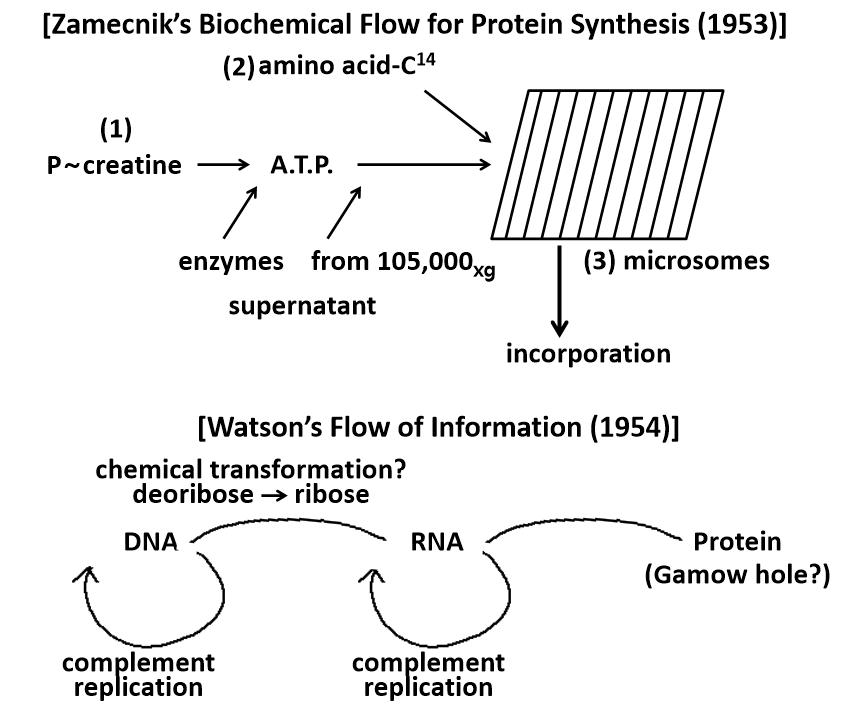
\includegraphics[width=.75\textwidth]{ART_Gim/fig.1_zamecnik_watson_bw.png}%
 \end{center}%
 \caption{Zamecnik and Watson's diagrams
 %\label{ref:RNDLYUtprlk80}(Judson, 2013, p.273)
 \parencite[based on][p.273]{judson_eighth_2013}}\label{gim.fig1}
\end{figure}

\begin{figure}[H]
 \begin{center}
 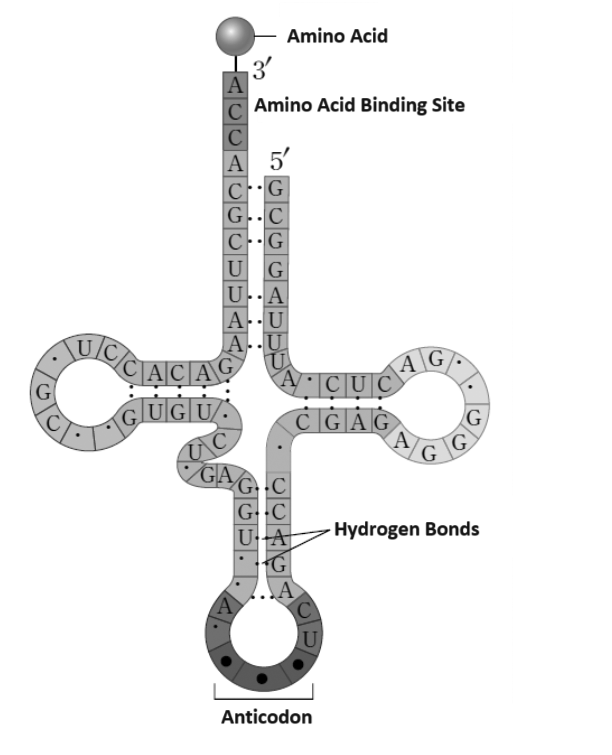
\includegraphics[width=.5\textwidth]{ART_Gim/fig.2_tRNA_bw.png}%
 \end{center}%
 \caption{The two-dimensional representations of tRNA
 %\label{ref:RND105yKmHiMv}(Holley et al., 1965, p.1464)
 \parencite[based on][p.1464]{holley_structure_1965}}\label{gim.fig2}
\end{figure}

\begin{figure}[H]
 \begin{center}
 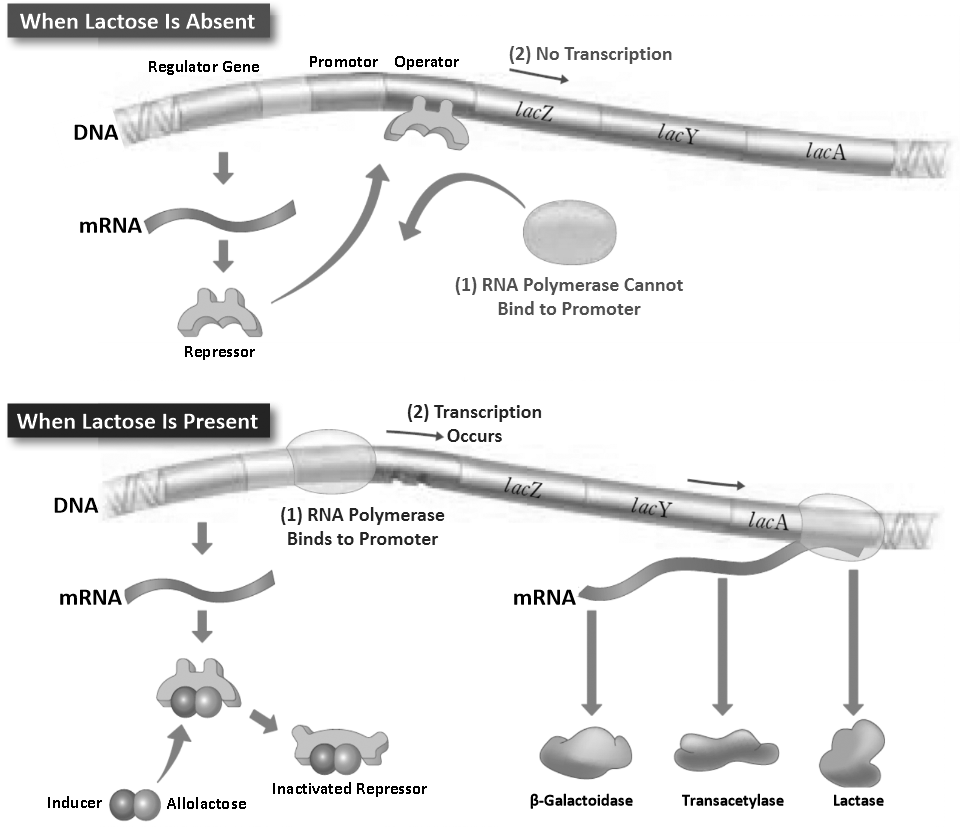
\includegraphics[width=\textwidth]{ART_Gim/fig.3_repressor_bw.png}%
 \end{center}%
 \caption[Models of the regulation of protein synthesis (based on Jacob and Monod, 1961, p.344)]{Models of the regulation of protein synthesis
 %\label{ref:RNDmyRLd6z9DD}(Jacob and Monod, 1961, p.344)
 \parencite[based on][p.344]{jacob_genetic_1961}\footnotemark\label{gim.fig3}
 }
\end{figure}
 \footnotetext{The regulation of gene expression in prokaryotes transpires at the transcriptional step. Multiple genes with analogous functions may be conglomerated into a singular transcriptional unit, thereby co-regulating their expression. This collective entity is denoted as an \textit{operon}, comprising a promoter, an operator region, and structural genes. The promoter serves as the site where RNA polymerase binds, initiating the transcription process. Simultaneously, the operator region, where a repressor protein is implicated in the regulation of transcription, spatially overlaps with the promoter, impeding RNA polymerase binding when the repressor protein is present. The structural genes encapsulate information pertaining to the proteins of three enzymes---$\beta $-galactosidase, transacetylase, and lactase---indispensable for lactose utilization. These three enzyme genes are collectively regulated within a singular operon, commonly known as the lactose operon. Expression of the lactose operon remains quiescent in the absence of lactose as a carbon source. Furthermore, even in the presence of lactose, expression ensues solely when a more favorable carbon source, such as glucose, is unavailable. The regulatory process unfolds sequentially: (1) In the absence of lactose, a repressor protein binds to the operator region, impeding transcription within the lactose operon. (2) Conversely, in the presence of lactose, the lactose inducer, allolactose, binds to the repressor protein, instigating a conformational alteration that precludes its binding to the operator region, thereby facilitating transcription within the lactose operon
 \parencite[for more details see][]{jacob_genetic_1961}.}
 
\begin{figure}[H]
 \begin{center}
 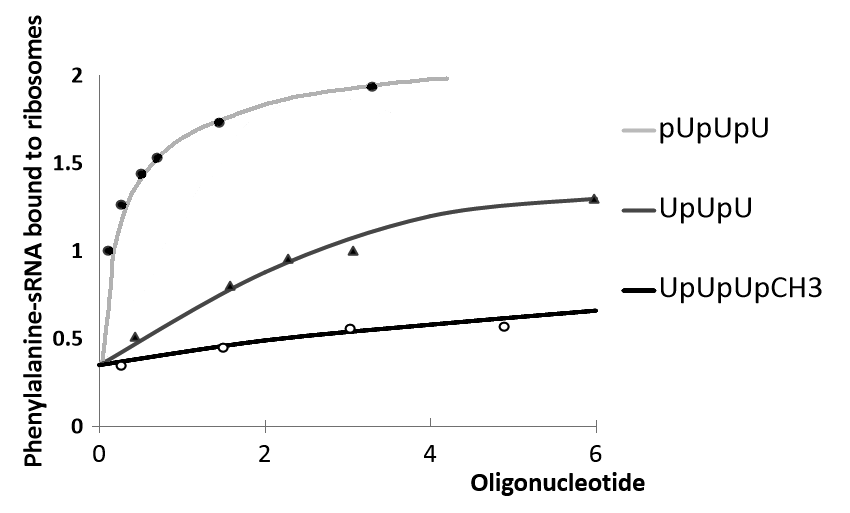
\includegraphics[width=.8\textwidth]{ART_Gim/fig.4_polyU_new_bw.png}%
 \end{center}%
 \caption{Effect of poly-U nucleotides with terminal phosphate on activities of synthesizing Phenylalanine
 %\label{ref:RND3bJIdkkvdG}(Rottman and Nirenberg, 1966, p.562)
 \parencite[based on][p.562]{rottman_rna_1966}}\label{gim.fig4}
\end{figure}


After determining the phenomenon to be explained, researchers hypothesize what objects are relevant to the phenomenon. They either formulate hypotheses about the relations between candidate objects or conduct experiments to identify whether the phenomenon occurs due to chemical interactions between objects. Watson, in 1954, and Crick, in 1958, proposed the RNA template hypothesis between DNA and protein based on existing results at that time. Zamecnik conjectured that a~ribonucleoprotein particle, later named a~‘ribosome,' within the microsome is engaged with protein synthesis
%\label{ref:RNDE4BJ8THx2q}(Hoagland et al., 1958).
\parencite[][]{hoagland_soluble_1958}. %
 The most famous experiment in molecular biology, the so-called PaJaMo experiment, performed by Arthur Pardee, Jacob, and Monod 
%\label{ref:RNDXG0NC4F3Pv}(1959),
\parencite*[][]{pardee_genetic_1959}, %
 implies DNA itself is not a~direct template of protein synthesis. Other biologists, including Severo Ochoa, Marshall Nirenberg, and Har Gobind Khorana, contributed to explaining how genetic information is transferred from one molecule to another.\footnote{Ochoa was a~Nobel Prize winner in 1959 for their discovery of the mechanisms in the biological synthesis of ribonucleic acid. Nirenberg and Khorana were also Nobel Prize winners in 1968 for their interpretation of the genetic code and its function in protein synthesis.}

Those theoretical or experimental results play a~crucial role in explaining the phenomenon of protein formation in distinct ways. Watson and Crick's RNA template hypothesis represents the genetic flow from DNA to protein via messenger RNA. This hypothesis is instrumental in explaining how DNA's genetic information is transferred to proteins. Zamecnik's diagram delineates the biochemical flow for protein synthesis utilizing the formation of ATP. This diagram proves useful in explaining the energetic components required in protein synthesis (see Fig. \ref{gim.fig1}). Holley's two-dimensional scheme from 1965 represents the structural shape of alanine RNA. This schematic representation is valuable in explaining how free amino acids are transported into the formation of polypeptides (see Fig. \ref{gim.fig2}). Jacob and Monod's models from 1961 illustrating the regulation of protein synthesis represent the interaction between regulator, operator, and structural genes. These models are effective tools in explaining how different genes contribute to synthesizing transcribed RNA (see Fig. \ref{gim.fig3}). Nirenberg's model of data shows that 5'-terminal phosphate poly-uracil sequences are more active in synthesizing phenylalanine linkages than in other sequence cases. This model is utilized to explain the structural features of mRNA required to form polypeptide linkages (see Fig. \ref{gim.fig4}).

It's important to note that researchers characterize the phenomenon of protein synthesis based on their individual interests. Molecular biologists, for instance, concentrate on genetic mappings from DNA to protein, while biochemists explore different facets of the phenomenon, such as energetic aspects (Zamecnik), structural analysis (Holley), enzymatic processes (Ochoa, Jacob \& Monod), and reaction rates (Nirenberg). Their research interests guide the representation of relevant parts of the protein synthesis mechanism. Watson and Crick, for example, speculated on the existence of messenger RNA between DNA and protein, while other biochemists employed various experimental instruments and interpreted data models. Some outcomes represent temporal steps of the mechanism, while others focus on the structural features of specific components. These diverse results prove valuable in explaining how proteins are formed in a~cell. In essence, most representations serve as worthy explanans for mechanistic explanations when used to depict the physical features of candidate parts, revealing their structural shape and considering them as relevant components. In a~nutshell, ``A researcher \textit{uses} linguistic and diagrammatic \textit{representations} of relevant parts and their organizational features of a~\textit{mechanism} to \textit{explain} a~phenomenon depending on the researcher's interests.''

Certainly, it is crucial to closely identify the relevant parts and their organizational features that are intricately linked to the occurrence of the explanandum phenomenon. However, the judgments regarding whether certain parts or organizational features are pertinent to the occurrence of the explanandum phenomenon are not issues within the conceptual dimension of explanation but rather fall under the relational dimension of explanatoriness. Here, I~emphasize that explaining a~phenomenon is conceptually identical to representing something that produces the phenomenon, and that representations are not binary but tertiary relations involving linguistic or non-linguistic representations, target entities or their organizations in the world, and human agents. These two emphases form the foundation for subsequent discussions about the relational and normative dimensions of the ontic-epistemic debates.

\section{On the explanatoriness of mechanistic explanation: Sufficiency vs. necessity}
As noted, Salmon has led us to consider mechanistic explanation as an alternative to Hempel's covering law model, presenting it as the ontic conception of explanation, in contrast to the epistemically inferential nature of the latter. In the original ontic-epistemic debate, it is well-known that Hempel's model faces numerous counterexamples, as detailed in Section 2. Consequently, many proponents of the New Mechanism, including Bechtel, argue that mechanistic explanation naturally falls into the ontic realm within the relational dimension of explanation.

However, caution is warranted because the prioritization of the ontic conception of explanation against Hempel's viewpoint is situated within the dimension of explanatoriness. I~previously underscored the importance of representation in understanding the nature of explanation within the conceptual dimension. Herein, several questions arise. If we adopt an epistemic position in the conceptual dimension of the nature of explanation, are we compelled to align with Hempel's viewpoint in the dimension of explanatoriness once again? If not, does that imply a~rejection of Hempel's ideas? Suppose we choose not to adhere to Hempel's inferential version of the epistemic account of explanatoriness. How can we maintain a~non-ontic position of explanation within the dimension of explanatoriness? Furthermore, how compatible are the two epistemic positions in the two dimensions - explanatoriness and the nature of explanation - with each other?

One of the most fatal shortcomings in Hempel's model is that his conditions for scientific explanation are insufficient in the relational dimension of explanatoriness. For instance, the flagpole or eclipse case serves as a~counterexample to the condition of the explanatory form, which is an argument. The barometer case functions as a~counterexample to the condition of the explanatory force, whether it be universal or probabilistic laws. The contraceptive pill case serves as a~counterexample to the explanatory relevance condition, which is a~logical necessity. Similarly, the vitamin C~case is a~counterexample to the condition of explanatory relevance based on high probability. These counterexamples demonstrate that arguments, laws of nature, logical necessity, and high probability alone are insufficient for scientific explanations. I~pursue a~way to adopt the epistemic position of \textit{mechanistic} explanation in the relational dimension without falling into the swamp that Hempel's model confronted.

My primary strategy to advocate the epistemic view of mechanistic explanation does not involve searching for other ideal conditions of scientific \textit{explanation}, as Hempel did. Instead, I~will regard Hempel's covering law model as a~pursuit of \textit{necessary} conditions for scientific \textit{representation}, assuming that mechanistic explanations are representations relative to pragmatic interests. In other words, Hempel's four conditions are necessary for the format of representations of mechanisms in the context of ``An \textit{agent} uses \textit{linguistic representations} to depict \textit{mechanisms} to \textit{explain} the explanandum-phenomenon.'' If some descriptions of a~mechanism fail to satisfy Hempel's conditions, then the linguistic representations of the mechanism are also deemed inadequate.

Let me begin with a~question: Are all linguistic representations, such as statements, propositions, and descriptions, inadequate for depicting mechanisms? Bechtel and Abrahamsen
%\label{ref:RNDI3rRLl63MZ}(2005)
\parencite*[][]{bechtel_explanation_2005} %
 seem to prioritize non-linguistic representations of mechanistic explanations. However, I~do not intend to discuss the priority of representational forms here. Instead, I~presume that linguistic and diagrammatic representations are essential modes of mechanistic explanation. Although many mechanistic explanations are diagrammatic, they never completely replace all linguistic expressions. Instead, linguistic descriptions support us in illustrating spatiotemporal processes of mechanisms, understanding detailed information, and communicating with diagrams. Most philosophers of science who advocate the New Mechanism believe that diagrammatic representations are primary modes of mechanistic models. Still, I~will concentrate on linguistic representations of mechanisms.

\subsection{Validity as a~necessary condition of linguistic representations}

As to the first condition about explanatory form, I~suggest adopting Hempel's first condition for linguistic representations of mechanisms, not for qualifying or eligible provisos of scientific explanation. I~never intend to advocate Hempel's model as an account of scientific explanation. I~am in alliance with the mainstream to criticize Hempel's covering law model. However, I~will deal with Hempel's conditions of \textit{linguistic representations} to satisfy them. My starting point was the dimension of the nature of mechanistic explanation. If we seriously take the epistemic conception of the nature of mechanistic explanation being representations, I~think Hempel's conditions help satisfy the necessary conditions for linguistic statements. In other words, all statements must be true, and an argument must be deductively valid.

In the case of protein synthesis, the ontic theorists may believe that facts, including transcription from DNA to mRNA and subsequent translation from mRNA to protein, explain how a~protein is synthesized from genetic materials. However, there seems to be a~wide gap between the belief that an actual mechanism exists and the observational evidence needed to justify that belief. No biologists directly observe the entire process from DNA to protein via mRNA. Strictly speaking, the mechanism of protein synthesis is unobservable. All processes of protein synthesis are inevitably decomposed and discovered separately in different laboratories. The results of experiments conducted on protein synthesis in each laboratory can be briefly summarized \textit{verbally}. For instance, Roger Kornberg observed a~specific case of transcription: an RNA polymerase synthesizes an mRNA sequence from DNA in a~eukaryotic cell. Marshall Nirenberg and Heinrich Matthaei observed a~particular case of translation such that a~typical complex of ribosomes and additional components synthesizes a~polypeptide containing only phenylalanine from a~poly-uracil sequence that is artificially composed by sole uracil. We can abstractly imagine that Kornberg's mRNA and Nirenberg's poly-uracil sequence are theoretically equivalent because both are a~single strand of nucleotide synthesized by an RNA polymerase in principle within a~typical environment. Under this theoretical condition, the two observations can be integrated into a~productively continuous process from DNA to protein via mRNA. Of course, diagrammatic representations are more intuitive to figure out detailed occurrences within both processes, but linguistic expressions are also possible as follows:

\begin{itemize}
    \item[\textit{C}\textit{\textsubscript{1}}.] Macromolecules, including DNA, mRNA, and protein, exist in a~eukaryotic cell.
    \item[\textit{C}\textit{\textsubscript{2}}.] Enzymes, including RNA polymerase and a~complex of ribosomes, also exist in eukaryotic cells.
    \item[\textit{P}\textit{\textsubscript{1}}.] An RNA polymerase synthesizes a~single nucleotide (mRNA) strand from DNA.
    \item[\textit{P}\textit{\textsubscript{2}}.] A~complex of ribosomes synthesizes a~primary sequence of proteins from mRNA.
    \item[\textit{C}\textit{\textsubscript{3}}.] mRNA's physical properties are always invariant, independent of concrete syntheses.
    \item[\textit{C}\textit{\textsubscript{4}}.] A~transcribed mRNA is abstractly identical to a~template of translation in principle.
    \item[\textit{E}.] The product of proteins is produced from DNA via mRNA.
\end{itemize}


The two conditions C\textsubscript{1} and C\textsubscript{2} are true on the ground that Watson \& Crick's model of DNA, Wilkins \& Franklin's X-ray diffraction evidence, and Kornberg \& Nirenberg's experimental models. Crick's central dogma, DNA $\to$ mRNA $\to$ Protein, is filled with objects. The two premises, \textit{P}\textit{\textsubscript{1}} and \textit{P}\textit{\textsubscript{2}}, are also true in Kornberg and Nirenberg's research. That is, arrows in Crick's central dogma are filled with enzymes. The additional conditions, \textit{C}\textit{\textsubscript{3}} and \textit{C}\textit{\textsubscript{4}}, are essential to integrate separate transcription and translation. These additional conditions are not ontic but epistemic claims because they are based on abstractly regular patterns from empirical research findings. Without direct observations of the mechanism of protein synthesis, the explanandum-phenomenon, \textit{E}, is a~deductive consequence of initial conditions and premises. In other words, a~deductive structure between statements is essential for linguistic representations to be useful in explaining phenomena.

Note that the mechanistic explanation above is linguistic. Premises are expressed lawfully and include empirical contents. All statements must be true either empirically or in principle. Due to two conditions \textit{C}\textit{\textsubscript{3}} and \textit{C}\textit{\textsubscript{4}}, the conclusion, \textit{E}, can be derived from \textit{C}\textit{\textsubscript{1}}, \textit{C}\textit{\textsubscript{2}}, \textit{P}\textit{\textsubscript{1}}, and \textit{P}\textit{\textsubscript{2}}. Be cautious that I~never argue that the mechanistic explanation satisfies Hempel's covering law model. I~intend to show that mechanistic explanation can be expressed linguistically as well as diagrammatically, and that if expressed linguistically, it must suffice Hempel's condition of explanatory form. Validity is a~fundamental requirement of linguistic representations to be an argument. I~never deal with valid arguments as a~sufficient condition of scientific explanation. My focus is not on finding sufficient conditions of scientific explanation but on finding the necessary conditions of linguistic representations. In other words, Hempel's logical condition is a~\textit{necessary} \textit{instruction} of linguistic representations, not a~scientific explanation. If linguistic representations are not valid, then they are absurd and non-informative in the end.

\subsection{Laws as a~necessary condition of understanding for explanatory force}

The ontic theorists claim that universal laws (or highly probabilistic laws) are insufficient conditions for scientific explanation. I~agree. However, I~emphasize that laws of nature are \textit{necessary} to understand how activities (or component operations) are engaged with entities (or component parts) and how they are spatiotemporally organized.

According to the ontic view, only things and facts are explanatory. In the case of protein synthesis, DNA, mRNA, and proteins are relevant entities. Moreover, transcription from DNA to mRNA means that the genetic information of DNA is transmitted into that of mRNA. Translation from mRNA to protein is also a~factual process that determines the types of amino acids and their order based on the genetic information of mRNA. In Crick's central dogma, all pertinent objects (DNA, mRNA, protein) are discovered, and two sequential transitions are also identified empirically. A~question arises: Can we understand, with only those objective facts, how entities act in reactions, how activities occur, and how components are organized?

Most advocates of the New Mechanism, whether they are ontic or epistemic, believe that activities (or component operations) give explanatory forces. According to Machamer, Darden, and Craver
%\label{ref:RND81P1djvH39}(2000, p.14),
\parencite*[][p.14]{machamer_thinking_2000}, %
 there are four types of activities: (i) geometrical-mechanical, (ii) electro-chemical, (iii) energetic, and (iv) electromagnetic. I~will classify such activities in Table \ref{gim.tab1}.


\begin{table}[]
\resizebox{\textwidth}{!}{%
\begin{tabular}{@{}ll@{}}
\rowcolor[HTML]{CBCEFB} 
{\bfseries Type} &
{\bfseries Activities}\\
\rowcolor[HTML]{FFFFFF} 
Geometrical &
 Shaping\\
\rowcolor[HTML]{ECF4FF} 
Mechanical &
 Fitting, Colliding, Pushing, Pulling, Opening, Closing\\
 \rowcolor[HTML]{FFFFFF} 
 Electrical &
  Attracting, Repelling\\
 \rowcolor[HTML]{ECF4FF} 
 Chemical &
  Bonding, Breaking\\
  \rowcolor[HTML]{FFFFFF} 
   Energetic &
    Thermodynamic\\
   \rowcolor[HTML]{ECF4FF} 
   Electro-magnetic &
    Electrically Conducting\\
%PP \bottomrule
\end{tabular}%
}
\caption{Types of activities.}
\label{gim.tab1}
\end{table}

\begin{figure}[H]
 \begin{center}
 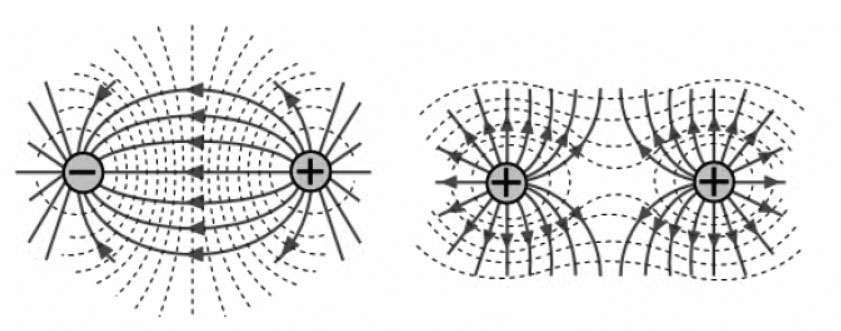
\includegraphics[width=.8\textwidth]{ART_Gim/fig.5300.jpg}%
 \end{center}%
 \caption{Attracting and repelling}\label{gim.fig5}
\end{figure}


As noted in Table \ref{gim.tab1}, activities are referred to as metaphorical terms. However, I~think that metaphorical terms are not fundamental foundations for providing explanatory forces because they must be elucidated under lower-level scientific theories. I~suggest metaphorical terms gain explanatory grounds when anchored in scientific facts, laws, or theories.

For example, electrical terms are based on Coulomb's law.\footnote{The potential energy, $\overrightarrow E(\overrightarrow r)$, of a~test charge $Q$ is the Coulombic energy of interaction between $Q$ and an arbitrary charge $q$ separated by a~distance $\overrightarrow r$ such that $\overrightarrow F(\overrightarrow r)=Q\overrightarrow E(\overrightarrow r)=Q\frac q{4\pi \varepsilon_0\overrightarrow r}$, where $\overrightarrow E(\overrightarrow r)$ is the electric force and $\varepsilon_0$ is the permittivity constant of vacuum.} Assume that atoms are the fundamental entity in our discussion.\footnote{This assumption is based on the atomic structure. All atoms consist of a~nucleus and one or more electrons. A~nucleus is electrically positive, whereas electrons are negative, so electric activities occur between them. There is attraction between the nucleus and the electrons, while there is repulsion between electrons. Repulsion also occurs between the nuclei of one atom and those of another atom adjacent to it. Electric activities are starting points to formalize entities and other activities because all materials contain a~nucleus and electrons.} Fig. \ref{gim.fig5} illustrates the explanatory ground of the electrical activities. The electrical field vector $\overrightarrow E(\overrightarrow r)$ is represented by lines pointing in the direction of the electric field at any point; that is, the electric field vector is tangent to the electric field lines at any point. The number of lines per unit area passing through a~surface perpendicular to the lines is proportional to the strength of the electric field in a~given region. For a~positive point charge, the lines radiate outward from a~point, whereas for a~negative point charge, the lines converge inward. The number of field lines leaving the positive charge equals the number of lines terminating at the negative charge. Fig. \ref{gim.fig5} illustrates the electric field lines for either two positive point charges or two negative point charges. The attraction and repulsion activities, describing the electrical interaction between charges, are mathematically formulated by Gauss' law.\footnote{The direction of electric flux is from a~positive point charge to a~negative point charge. In other words, electric flux, $\Phi _E$, is a~measure of the electric field vectors penetrating a~given surface. It is proportional to the number of field lines that pass through a~given region, $\overrightarrow A$, oriented perpendicular to the field, which is represented by the following equation: $\oint _S^{\Box} \overrightarrow E{\cdot}d\overrightarrow A=\Phi _E=\overrightarrow E\overrightarrow A\cos \theta $, where a~vector perpendicular to the region, $\overrightarrow A$, is at an angle $\theta $ concerning the field. The equation represents Gauss's law, ${\nabla}{\cdot}\overrightarrow E=\Phi _E=\frac Q{\varepsilon _0}$. Gauss's law implies that the electric flux through any closed surface is equal to the net charge inside the surface $Q$ divided by $\varepsilon _0$. Gauss' law is a~fundamental ground for the electrical activities.}

What about chemical activities? Those activities are also based on laws and theoretical backgrounds in physics. The two activities based on Coulomb's and Gauss's laws play a~fundamental role in constructing molecules with interactions between the nucleus and the electrons of atoms. The second step in constructing molecules is to examine the \textit{chemical} activity relating to how atoms combine in a~molecule. A~molecule comprises more than two atoms that share electrons. Covalent bonding is the most potent chemical bond when atoms share electrons. Molecular orbital theory (MO theory) is a~widely accepted theory to explain how covalent bonding occurs. Further, the Schrödinger equation can be solved analytically only for H\textsuperscript{+}\textsubscript{2}, but the solution cannot be applied to hetero-polyatomic molecules. In MO theory, the linear combination of atomic orbitals (LCAO) is an algebraic method to calculate the overall wavefunctions of electrons within a~molecule.\footnote{An atomic orbital is a~wave function that describes the behavior of an electron within an atom. Molecular orbitals can be calculated using the available atomic orbitals within various chemical contexts. (i) Electrons supplied by the atoms are accommodated in the orbitals to achieve the lowest overall energy, adhering to the constraints of the Pauli exclusion principle, which states that no more than two electrons may occupy a~single orbital, and they must be paired. (ii) If several degenerate molecular orbitals are available, electrons are added singly to each orbital before doubly occupying any one orbital because that minimizes electron-electron repulsions. (iii) Hund's rule implies that if two electrons occupy different degenerate orbitals, a~lower energy is obtained if they do so with parallel spins. In short, the structure of a~molecule is determined by the configuration of electrons within the molecules under the minimal energetic state. All these descriptions of physicochemical backgrounds are prepared with reference to Atkins and de Paula's Physical Chemistry textbooks
%\label{ref:RNDfgHGFjtinW}(see Atkins, De Paula and Friedman, 2014).
\parencite[see][]{atkins_physical_2014}.%
}

Hence, laws and theoretical backgrounds provide a~scientific understanding of why metaphorical terms are explanatory. I~do not argue that universal laws are a~sufficient condition of scientific explanation. Instead, I~emphasize the necessity of laws for an intellectually ultimate understanding of the explanandum phenomenon.

\subsection{Counterfactual inference as a~necessary condition of explanatory relevance}

Logical necessity is not a~sufficient condition for explanation. Even if an argument concludes the occurrence of a~phenomenon from sentences about relevant components and their organizational features is valid, the presence of a~sentence about an entity being causally inefficacious to the occurrence of the phenomenon in the premises renders the argument not a~mechanistic explanation. Moreover, no matter how much an inductive argument is based on high probability in the case of most prokaryotic cells, there is no guarantee that the argument will immediately apply to the case of eukaryotic cells. For this reason, Hempel's two conditions of explanatory relevance are deemed insufficient.

Assuming that explanations are representations, I~emphasize that Hempel's conditions should be considered necessary but insufficient. As noted earlier, logical necessity is crucial when explaining a~phenomenon through a~set of linguistic descriptions. It serves as a~prerequisite for the explanatory form rather than a~condition guaranteeing explanatory relevance. Within Hempel's account of explanation, there are no adequate conditions for mechanistic explanation.

Alternatively, I~introduce an inference to affirm the relationship of constitutive relevance between the explanandum phenomenon and descriptions of parts and organizational features: \textit{counterfactual conditional}.\footnote{In most cases of biological mechanisms, descriptions of the explanandum phenomenon are at a~higher level than descriptions of component parts and their activities. Advocates of the New Mechanism, particularly Craver, regard explanatory relevance in mechanistic explanation as \textit{constitutive} relevance. Although the philosophical debate remains, we will tentatively assume here that the two concepts of relevance are identical.} All phenomena to be ontologically explained depend on their lower-level mechanisms. This ontological dependence can be linguistically reformulated by a~‘because' complex sentence. To ensure explanatory relevance in the relational dimension, it must be demonstrated that the statement ‘The description of the phenomenon clause (P) is true because a~set of descriptions of mechanism clauses (M) is true.' The truth conditions of this sentence are provided by the counterfactual condition, stating that ‘P-clause because M-clauses' is true if and only if: (i) ‘P-clause' is true, (ii) all ‘M-clauses' are true, and (iii) ‘If it were not the case that M, it would not be the case that P' is true.\footnote{This kind of formal investigation of the explanatory relationship based on the ‘because' complex sentence has been slightly shown in Wright and Bechtel's paper in 2006. However, they did not formulate their idea at all. I~will adopt the counterfactual truth conditions of the ‘because' sentence as an epistemic condition of counterfactual inference for explanatory relevance. They said, ``Descriptions of mechanisms are not just coincident with, or derivative from, explanations -- they \textit{are} explanations. But explanations are not merely lists of descriptions of mechanisms or sets thereof: they include inferential and simulatory operations on them. (Considerations of the semantics of the explanatory connective ‘because', as well as what it is that arrow in box-and-arrow diagrams represent, help in grasping this point.)''
%\label{ref:RND0o2wh99B14}(Wright and Bechtel, 2007, p.53, emphasis original).
\parencite[][emphasis original]{wright_mechanisms_2007}. %
 I~will develop their basic idea by pursuing counterfactual conditions of the ‘because' sentence.}

A~sentence ‘P because M' indicates the explanatory relevance of mechanistic explanation between the explanandum phenomenon and explanans, assuming that every phenomenon (P-clause) depends on its mechanisms (M-clauses). Suppose a~description within the P-clause is false. In that case, all claims of explanatory relevance are false, as the first condition is not satisfied, regardless of the truth of the descriptions of mechanisms. It highlights that characterizing the explanandum phenomenon by determining its initial and terminal conditions is the primary cognitive activity of explanation. Similarly, if a~description within the mechanism clauses is false, the ‘because' sentence also becomes false, as the second condition is not satisfied, irrespective of the truth of the phenomenon description. These considerations presuppose that mechanistic explanation is a~cognitive activity in the first conceptual dimension of explanation. It is important to note that some explanations can be false due to misrepresentations, not the non-existence of relevant components and their organizational features.

The third truth condition is crucial in judging the relevance between P~and M~descriptions. Let's assume that M~is a~description of a~candidate for the relevant part of a~mechanism. If the occurrence of the P-description is observed even when it is not the case that M~($\sim$M), then it is certain that the referent in M~is irrelevant. The counterfactual conditional ``If it were not M, it would have been P'' is false since the P-description is true even if the M-description is false. For instance, from the molecular biologists' perspective, let me first discuss a~linguistic description of M-clause: ``X is a~genetic intermediate between DNA and protein'' (M\textsubscript{1}). Suppose a~biologist makes M\textsubscript{1} by filling the description with ribosomal RNA within a~microsome. In that case, ribosomal RNA is not relevant because it has been proven that protein synthesis occurs even if M\textsubscript{1} is false. On the other hand, suppose another biologist makes M\textsubscript{1} by filling the description with messenger RNA. In this case, the counterfactual conditional ``If it were not M\textsubscript{1}, it would have been not P'' is true since protein synthesis cannot be realized without mRNA.

It should be noted that we are not suggesting here that ribosomal RNA is an entirely incorrect component in protein synthesis. Rater, We found that ribosomal RNA was not an appropriate referent in the mechanistic description, ``\textit{X} is a~genetic intermediate between DNA and protein.'' Ribosomal RNA is the correct referent for other mechanistic descriptions, such as ``\textit{X} synthesizes polypeptides based on messenger RNA sequence'' (M\textsubscript{2}). In other words, it is not realistic to determine whether a~single referent is correct or incorrect for an entire mechanism. A~referent may be correct for a~description in one context and may be incorrect for other descriptions in another context.\footnote{Reversely, the occurrence of the P-description may not be observed even if a~mechanism description is true. In this case, the counterfactual condition ``If it were M, it would have been $\sim$P'' is false so that the mechanism description includes irrelevant information. Here, all true mechanism descriptions can be proven as totally irrelevant to the phenomenon because all referents and their properties in M-clauses never contribute to generate the occurrence of the phenomenon. As a~result, we easily ignore all such mechanism descriptions.}

Additionally, from the biochemists' point of view, let me focus on enzymatic activities, particularly RNA polymerase. The counterfactual inference is well applicable to cases of step-by-step processes. An RNA polymerase is a~key entity synthesizing mRNA with DNA. When explaining the production of mRNA, ontic theorists may provide a~mechanistic explanation as follows. Suppose that an explanandum-phenomenon, \textit{P}, is the production of mRNA sequence through transcription. The emergence of mRNA is the terminal outcome of the mechanism of RNA synthesis. The initial condition of the production is nothing of any ribonucleic acids in a~cell's nucleus. However, we must assume that there are a~lot of building units of the mRNA, including adenine, uracil, guanine, and cytosine. A~M-clause is ``mRNA sequence emerges in a~cell's nucleus.'' The truth condition of the M-clause could be determined by empirical manipulation like centrifugal identification. In the 1960s, the existence of mRNA was proven by Brenner et al. What are the M-clauses as explanans of the P-clause? Briefly speaking, there are five statements of the M-clauses as follows:

\begin{itemize}
    \item[M\textsubscript{3}.] An RNA polymerase attaches a~DNA region called the promoter sequence.
    \item[M\textsubscript{4}.] The RNA polymerase unwinds the two strands of DNA.
    \item[M\textsubscript{5}.] The RNA polymerase moves along the DNA.
    \item[M\textsubscript{6}.] At that time, the RNA polymerase synthesizes individual RNA nucleotides to the growing mRNA strand based on a~single strand of DNA template.
    \item[M\textsubscript{7}.] The RNA polymerase detaches from the DNA template when stopping the synthesis.
\end{itemize}
\enlargethispage{1.5\baselineskip}


If M\textsubscript{6} is not true, the P-description, ``A transcription is generated,'' may also not be true since M\textsubscript{6} implies the P-description. M\textsubscript{6}~temporally depends on M\textsubscript{5}, which also depends on M\textsubscript{4}, which depends on M\textsubscript{3}. M\textsubscript{7} indicates the end of the series from M\textsubscript{3} to M\textsubscript{6}. As a~result, if a~sequence of successive M-descriptions is false, then the P-description as a~consequence of the terminal M-description is also false. That is, if M\textsubscript{3}$\sim$M\textsubscript{7} is not true, then P~is not true, too. In conclusion, M-descriptions, M\textsubscript{3}$\sim$M\textsubscript{7}, are explanatory relevance to the P-description. An inference with the counterfactual conditional is worthy of being an adequate epistemic condition to discern whether any mechanistic descriptions are relevant to the phenomenon description.

Finally, I~do not argue the structural identity between mechanistic explanation and prediction. We do never adopt the demarcation problem because prediction is an explanatory virtue. Hempel's four conditions are insufficient for scientific explanations to satisfy but necessary to evaluate whether linguistic representations are adequate. No matter how logical necessity (or high probabilistic necessity) is satisfied from the premises and their conclusion, it does not guarantee that linguistic representations are scientific explanations. However, if all statements are employed to explain something, they must be logically consistent. If not so, independently of whether logical necessity is a~sufficient condition to determine the eligibility of scientific explanation, all linguistic representations are not informative. Moreover, laws of nature are not sufficient conditions for scientific explanations. However, in the absence of laws of nature, it is difficult to identify the explanandum phenomenon and further understand how organizational features of mechanisms contribute to producing the occurrence of the phenomenon.

Hempel's account is epistemic because epistemic inferences, such as logical calculus or derivations, establish explanatory relevance. In contrast, Salmon's causal-mechanical account is ontic because explanatory relevance is established not by mental inferences based on logic but by actual target systems in nature, expected to bring about a~phenomenon to be explained. Attempts to evade Hempel's shadow were unsuccessful in establishing the epistemic view in the relational dimension of explanatoriness in the original ontic-epistemic debate.

To advocate the epistemic conception of mechanistic explanation, I~propose two epistemic ways to illuminate the explanatory relevance between the explanandum phenomenon and its explanans: the necessity thesis of linguistic representations and the counterfactual inference. Hempel's epistemic conditions are necessary for mechanistic explanations, which are linguistic outcomes representing actual mechanisms under the assumption that linguistic descriptions express the contents of mechanistic explanation. Additionally, a~counterfactual inference of the ‘because' sentence helps check whether the relation between the explanandum and explanans is relevant. I~illustrate this with molecular and biochemical cases. These alternative interpretations of Hempel's account of explanation in the relational dimension of explanatoriness are based on the previous consequence that the nature of explanation is a~cognitive activity in the conceptual dimension.

\section{On the norms of mechanistic explanation: Completeness vs. purpose-dependence}
\enlargethispage{1.5\baselineskip}
Most philosophers have discussed the normative dimension by emphasizing the superiority or interaction between ontic and epistemic norms
%\label{ref:RND0BmXWK6A6a}(Kaplan and Craver, 2011; Illari, 2013; van Eck, 2015; Sheredos, 2016).
\parencites[][]{kaplan_explanatory_2011}[][]{illari_mechanistic_2013}[][]{van_eck_reconciling_2015}[][]{sheredos_re-reconciling_2016}. %
 In contrast, I~will focus in this Section on these two types of norms as criteria for evaluating mechanistic explanations. Many ontic theorists defend ontic norms by mentioning that ontic norms are the most powerful standard for evaluating explanations 
%\label{ref:RNDn576ysYLyz}(see Craver, 2014; Povich, 2018).
\parencites[see][]{kaiser_ontic_2014}[][]{povich_minimal_2018}. %
 Participating in the ontic-epistemic debate as a~standard for evaluating mechanism explanations is noteworthy since it is an issue of the normative dimension of explanation that has yet to receive much attention among epistemic advocates. However, I~would like to point out that, contrary to the wishes of ontic theorists, when they use ontic norms when evaluating mechanistic explanations, they encounter dilemmas that run counter to our common sense.

\subsection{Pessimistic induction and demarcation of explanation}

If we adopt the idea that mechanistic explanation is a~cognitive achievement to represent a~mechanism linguistically or diagrammatically in the conceptual dimension, what implications does it have for normative issues? Generally, mechanists refer to representations of mechanisms as mechanism schemes. Assuming this equivalence of abstract two terms, we can say that Craver emphasizes two ontic norms of mechanistic explanation: (i) completeness and (ii) correctness. He, with Darden, defines the two terms as critical criteria to evaluate mechanism schemes
%\label{ref:RNDeBt3Hf36sc}(Craver and Darden, 2013, p.9):
\parencite[][p.9]{craver_search_2013}: %
 ``Completeness presumes that there is a~complete target mechanism in the world, and one can assess the extent to which the schema includes all and only the entities, activities, and organizational features in the target. Correctness presumes that there is a~fully instantiated target mechanism in the world, and one can assess the degree of fit or mapping between items in the scheme and items in the target mechanism.'' As noted previously, completeness is a~chief ontic goal of mechanistic explanation. Correctness is closely related to Craver \& Kaplan's 3M requirement between a~scheme and its target mechanism.

Note that most ontic theorists, including Craver, Kaplan, and Povich, further employ those ontic norms to demarcate good from bad explanations. Ontic theorists seem to believe that a~philosophical search for any criteria to evaluate the quality of explanation is a~critical task of the philosophers of science. They think of mechanism sketches (or how-possibly models) as mere conjectures of the target. On the other hand, they appear confident that we can attain correct and complete representations of the entire target mechanism as how-actually models. They tend to regard mathematical descriptions of natural patterns as trifling or partial explanations. Hodgkin and Huxley's equations of action potential are the typical case. No matter how the equations allude to regular patterns across a~membrane of a~neuron quantitively, ontic theorists underestimate the explanatory values of mathematical descriptions
%\label{ref:RNDeGOFEod5W7}(see Craver, 2007).
\parencite[see][]{craver_explaining_2007}. %
 They stress the significance of only qualitative descriptions (or diagrams) with causal terms within Table \ref{gim.tab1}. They seem to believe that referring to relevant components and their organizational patterns is the superior prerequisite of mechanistic explanation than depicting them mathematically.

\enlargethispage{1.5\baselineskip}
Let's delve into ontic norms by addressing the following questions: Is the ontic norm of completeness attainable? How can we determine whether completeness is achieved without prior knowledge of the target mechanism? These inquiries pose metaphysical doubts about ontic norms. Moreover, most mechanism schemes are inevitably labeled as bad explanations when completeness is employed as a~criterion for evaluation. The question then arises: Should we rely on completeness to distinguish between good and bad explanations?

Firstly, is the ontic norm of completeness applicable to the evaluation of hypothetical mechanism schemes? According to Craver \& Darden's definition of completeness, an agent must possess complete information about a~target mechanism before employing this ontic norm. This comprehensive information includes the types of entities, activities, and their organizational features. However, completeness is an unattainable criterion when applied to practical contexts. Information about the target must be known in advance to use the completeness norm in evaluation. Yet, as demonstrated earlier, direct access to a~target mechanism is not feasible. We cannot grasp information about mechanisms all at once, and scientific instruments do not aid in perceiving the entire process of the explanandum phenomenon. Instead, we must partially grasp mosaic information about the mechanism and then piece the information together.\footnote{Craver emphasizes the mosaic unity in neuroscience for a~different reason
%\label{ref:RNDpnY1dXT2yg}(see Craver, 2007).
\parencite[see][]{craver_explaining_2007}. %
 He argues that mechanistic explanations in neuroscience are not reduced to the fundamental level but are unified by multilevel results of different fields.} Completeness is not a~tangible concept that can be achieved in one fell swoop. Instead, it is a~variable concept that gradually changes in magnitude and degree as the obtained evidence increases.

Second, completeness is not an appropriate criterion for evaluating whether an explanatory representation is good or bad. This ontic constraint is a~variable concept depending on how far the research has progressed. Is Crick's central dogma, DNA $\to$ RNA $\to$ Protein, a~mechanism scheme? Most ontic theorists seem to answer yes because the missing link was filled with RNA. Further, this scheme opens the way to explain how proteins are synthesized from DNA. However, this mechanism scheme seems to be a~bad explanation under the completeness criterion because the scheme does not include which enzymes act when RNA is transcribed from DNA and when protein is translated from RNA. Perhaps ontic theorists believe a~complete explanation can be achieved by enumerating the complex processes by which RNA and protein are synthesized separately, using causal terms. Or they may believe that a~complete explanation can be more easily achieved if the two syntheses are presented concisely, using diagrams.

Perhaps ontic theorists would say this is on the way to complete a~mechanism description. Of course, pursuing completeness by adding unknown sub-processes in more detail than the previous mechanism descriptions is not problematic. The genuine problem arises from the fact that proposing a~mechanistic explanation depends on additional research findings. More novel components will be continuously discovered in pursuit of a~complete mechanism description. And new interactions between the components will also emerge. The additional achievements of these discoveries are typical of biological research, which is entirely natural. But do biologists always classify their explanations as good or bad based on the yardstick of completeness? That rarely happens. All of their explanations are on a~\textit{continuum}, and it is highly unrealistic to divide the sequence of achievements into good and bad explanations solely based on completeness.

\enlargethispage{1.5\baselineskip}
Let's reconsider the case of protein synthesis, particularly examining whether the mechanism schema in Fig. \ref{gim.fig6} serves as a~complete and correct model to represent the full processes of protein synthesis. Regrettably, the schema is inherently incomplete. Firstly, the discovery of reverse transcriptase in 1970 unveiled a~reverse flow of genetic information from an RNA virus to a~DNA provirus. Secondly, eukaryotic mRNA is not immediately ready for translation. RNA at this stage is termed precursor-mRNA and must undergo additional processing before transitioning from the nucleus to the cytoplasm as mature mRNA. These processes involve RNA capping, polyadenylation, and splicing, modifying mRNA in various ways. These modifications enable a~single gene to produce more than one protein.\footnote{RNA capping modifies the 5' end of the RNA transcript, which is the end that is synthesized first. RNA is capped by the addition of an atypical nucleotide, which is a~guanine nucleotide containing a~methyl group attached to the 5' end of RNA in an unusual way. This capping occurs after RNA polymerase II has produced about 25 RNA nucleotides long before completing transcription of the entire gene. Polyadenylation provides newly transcribed mRNA with a~special structure at the 3' end. Unlike bacteria, where the 3' end of an mRNA is simply the end of a~chain synthesized by RNA polymerase, the 3' end of a~eukaryotic mRNA is first trimmed by an enzyme that cleaves the RNA chain at a~specific sequence of nucleotides. The transcript is then finished by a~second enzyme that adds a~series of repeating adenine nucleotides to the cleavage ends. These poly-A tails are typically hundreds of nucleotides long. Splicing removes introns from precursor-mRNAs. Introns are unnecessary regions for encoding proteins. The rest of the mRNA consists only of regions called exons that are needed to synthesize the protein. Editing is the process of changing some nucleotides in mRNA. For example, a~human protein called APOB, which helps transport lipids in the blood, has two different forms due to editing. One form is smaller than the other because editing adds an earlier stop signal to the mRNA. RNA editing processes such as these occur all the time in real cells. In order for the mechanism by which RNA is synthesized from DNA to meet the criteria for completeness, an explanation including these processes is required.} Third, the full mRNA sequence after transcription is not the genetic code for synthesizing proteins. Precursor RNAs synthesized by an RNA polymerase in the nucleus must be edited. Particularly, the splicing mechanism in eukaryotes is essential; non-genetic portions within the precursor RNAs, the so-called introns, must be deleted, and genetic portions, the so-called exons, must be ligated. Splicing implies that both synthesizing processes, transcription, and translation, are not the only processes within protein synthesis. In other words, Fig. \ref{gim.fig6} is never a~complete model of protein synthesis.
\enlargethispage{1.5\baselineskip}

\begin{figure}[H]
 \begin{center}
 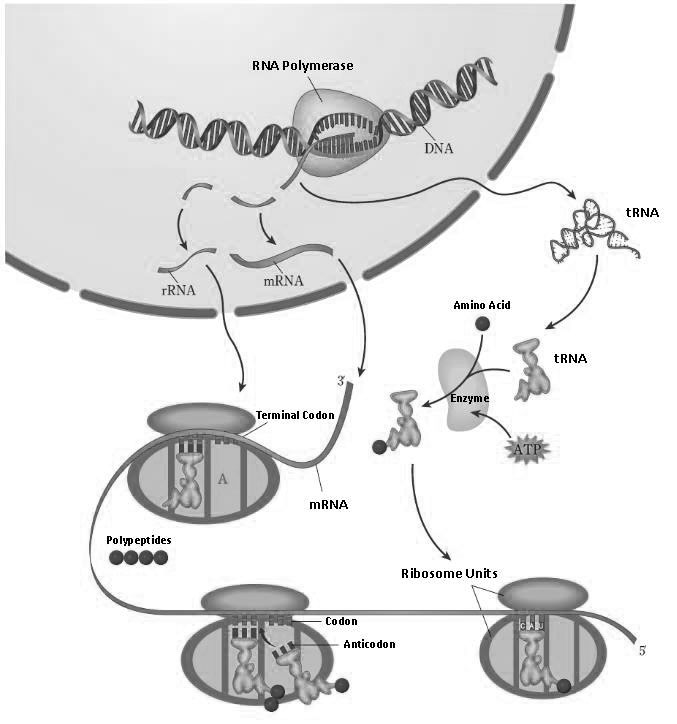
\includegraphics[width=.8\textwidth]{ART_Gim/fig.6_bw.jpg}%
 \end{center}%
 \caption{Mechanistic schema for protein synthesis
 %\label{ref:RND5ZkgEBeN2n}(Darden, 2006, p.117)
% \parencite[][p.117]{darden_reasoning_2006}
 }\label{gim.fig6}
\end{figure}

Maybe ontic theorists complain that those two cases, retrovirus and splicing reactions, do not refute their ontic norms to evaluate mechanism schemes because they are not counterexamples but evidence of their ontic criteria. The more processes are filled with the previous scheme, the more complete and correct explanations are achieved. Suppose that it is okay to accept the ontic theorists' claim such that the mechanism scheme, including (i) Watson's central dogma, (ii) biochemists' discoveries of enzymatic reactions from DNA to protein, (iii) a~special case of genetic information flow in a~retrovirus, and (iv) splicing mechanism in eukaryotes, is the complete and correct model of protein synthesis. Regrettably, again, Ochoa's discovery misrepresents RNA synthesis because he never found RNA polymerase but polynucleotide phosphorylase. Roger Kornberg successfully analyzes the structural features of RNA polymerase and its functions in eukaryotes in the early twentieth century. In other words, all mechanistic schemes in the absence of Roger Kornberg's achievements are certainly incomplete and incorrect.

Again, ontic theorists would complain that the system of mechanisms, up to and including Roger Kornberg's discovery, is a~complete and accurate model of protein synthesis. The problem with answering this way is that ontic theorists can never seem to qualify themselves as tools for evaluating mechanism schemes other than holding their ground. Whenever a~discovery emerges, the existing mechanism scheme becomes a~false description, and a~more complete and accurate explanation is achieved. As biologists' research accumulates, situations like this will occur more frequently in the future. It is clear, then, that any mechanism scheme currently believed to be complete and correct will one day become a~bad explanation. The ontic norms applied to evaluating explanations inevitably allow for such \textit{pessimistic} prospects in situations where theory propagation is the norm. In this scenario, we must reluctantly conclude that achieving a~complete and precise mechanism is an elusive goal, both at present and in the foreseeable future.

This conclusion is analogous to the conclusion of the pessimistic induction argument against scientific realism. The pessimistic induction argument shows that if past successful and truly accepted theories were false, we fail to believe the realist's claim that our currently successful theories are true because current theories will also be false as past successful theories were confronted. Similarly, if one adopts the realistic point of view of the existence of a~mechanism and admits that mechanism schemes are continuously developed toward more complete and more correct models, then it is skeptical to attain the complete and correct model of the mechanism.

Advocates of the ontic conception of explanation believe (i) that we can one day achieve complete and accurate mechanism descriptions and (ii) we must assess mechanism schemes under the ontic norms. However, suppose the two beliefs juxtapose with each other. In that case, we are inevitably unable to obtain complete and accurate mechanism descriptions, or we are forced to brand almost all known mechanism descriptions as bad. Ontic theorists accept that mechanistic models must be developed from how-possibly to how-actually models. Mechanism sketches become just how-possibly models when acquiring more complete and correct models. By filling in intermediate components between the initial and terminal conditions, mechanism sketches must be developed into more complete and correct schemes as how-actually models. Suppose one realizes the acquisition of a~complete and correct model of the explanandum phenomenon. In that case, the how-actually model is a~good explanation, and all the early sketchy how-possibly models become bad explanations. Note that both ontic norms of completeness and correctness are criteria for evaluating mechanistic schemes from a~\textit{realistic} point of view. Craver and Darden reveal their realistic stance by saying that:

\myquote{
At the most abstract level, mechanism schemas are evaluated in terms of their depth, their completeness, and their correctness. We discuss these dimensions of evaluation and some tests for evaluating a~schema along these dimensions. Our orientation toward these questions might be described as a~\textit{garden-variety realism} moderated by a~sensible pragmatism
%\label{ref:RNDOu4WvGgjRc}(Craver and Darden, 2013, p.9, emphasis added).
\parencite[][emphasis added]{craver_search_2013}.%
}
Craver and Darden
%\label{ref:RNDyFBT8TKnwf}(2013, p.94)
\parencite*[][p.94]{craver_search_2013} %
 emphasize the close relationship between an ontic norm such as correctness and realism: ``The difference between how-possibly, how-plausibly, and how-actually a~mechanism works is a~difference in correctness. Mechanists are garden-variety realists about such things: the goal is to describe correctly enough (to model or mirror more or less accurately) the relevant aspects of the mechanism under investigation.'' It is taken for granted that ontic norms are realistic criteria because they are based on the external existence of relevant entities and activities of the target mechanisms.

A~problem of ontic norms as criteria for evaluating mechanism schemes is that all past achievements of mechanism schemes are just bad and provisional explanations. In other words, this decision is so hasty that it raises the problem of treating all existing scientific achievements as useless and bad things. But such a~judgment is too extreme. Is the discovery that genes are passed from DNA to mRNA to proteins a~bad achievement? Are all the diagrams missing the splicing process a~bad diagram of how proteins are synthesized? Are all of Roger Kornberg's schemes where RNA polymerase is not named or omitted bad descriptions? No matter how imperfect or inaccurate these achievements may ultimately be, they must be our historically significant assets. It is very questionable whether these achievements are appropriately treated as useless or bad simply because they are not complete and accurate mechanism schematics.

To summarize, ontic proponents may accept that the mechanism of protein synthesis, like the diagram of Fig. \ref{gim.fig6}, explains the production of the primary sequences of proteins in molecular biology. Is this mechanism complete? If they think this mechanism is complete, this judgment is false because the splicing mechanism is ignored. If they think this mechanism is incomplete, then ontic norms seem sterile to distinguish how-actual from how-possible models. Ontic theorists believe that ontic norms such as correctness and completeness play a~role in demarcating good from bad explanations. Unfortunately, as long as they continue to hold on to this belief, ontic theorists end up labeling a~mechanistic scheme, considered a~very important biological achievement, as a~‘bad' explanation. This tragic situation has resulted from adhering to a~particular philosophical position, the ontic criteria for evaluating mechanism schemes. Regardless of whether the splicing mechanism was discovered, Fig. \ref{gim.fig6} is still a~good representation that explains a~fairly important phenomenon in protein synthesis.

\subsection{Ontic norms as methodological instructions}

Suppose ontic norms such as completeness are difficult to achieve, and it is problematic to classify incomplete mechanism schemes into bad explanations according to these norms. What role do these norms play? Suppose we need not seriously consider mechanism schemes to be tagged as good or bad. Ontic norms can motivate researchers to provide more advanced explanations than previous explanations of mechanisms. As noted, mechanistic explanation relies on mechanistic inquiries. Completeness plays an instruction in developing existing schemes by filling unidentified processes or illuminating known entities' uncovered properties.

Again, for instance, the self-splicing mechanism in eukaryotes was discovered after most processes within the mechanism of protein synthesis were known in the 1980s. When discovering the structure of DNA in 1953, Watson and Crick never acknowledged the two distinctions, exons and introns, within nucleic acids. Exons are portions that include genetic information, whereas introns do not. So, introns must be removed before a~ribosome synthesizes proteins based on the genetic sequences of mRNA. Thomas Cech discovered the splicing mechanisms in \textit{Tetrahymena} (see Fig. \ref{gim.fig7})
%\label{ref:RNDKM1pP6CS48}(Zaug, Grabowski and Cech, 1983).
\parencite[][]{zaug_autocatalytic_1983}. %
 Due to the discovery of splicing processes, understanding of protein synthesis has increased. Moreover, Cech discovered a~new property of RNA. Until the 1980s, most biochemists believed that all enzymes are proteins. However, while investigating the splicing mechanism, Cech was also aware of the enzymatic property of RNA molecules. That is, Cech shed light on a~novel fact that biological reactions from pre-rRNA to spliced rRNA occur in the absence of enzymes (see Fig. \ref{gim.fig7}). Cech 
%\label{ref:RNDcKN42rgx2z}(1986)
\parencite*[][]{cech_model_1986} %
 proved it experimentally so that he won the Nobel Prize in 1989. Cech's discovery of ribozyme, a~compound of RNA \& enzyme, contributes to making more complete lists of referents of enzymes in the world. Cech's achievements are totally compatible with the previous outcomes. Biologists investigate their research to explain biological phenomena at the molecular level more completely. Ontic norms are methodological instructions in mechanism inquiries.\footnote{Although I~only focus on completeness here, correctness is also an important ontic norm in mechanism inquiries. Without referring to referents as correct entities in a~mechanism, we cannot explain the explanandum phenomenon successfully.}

\begin{figure}[H]
 \begin{center}
 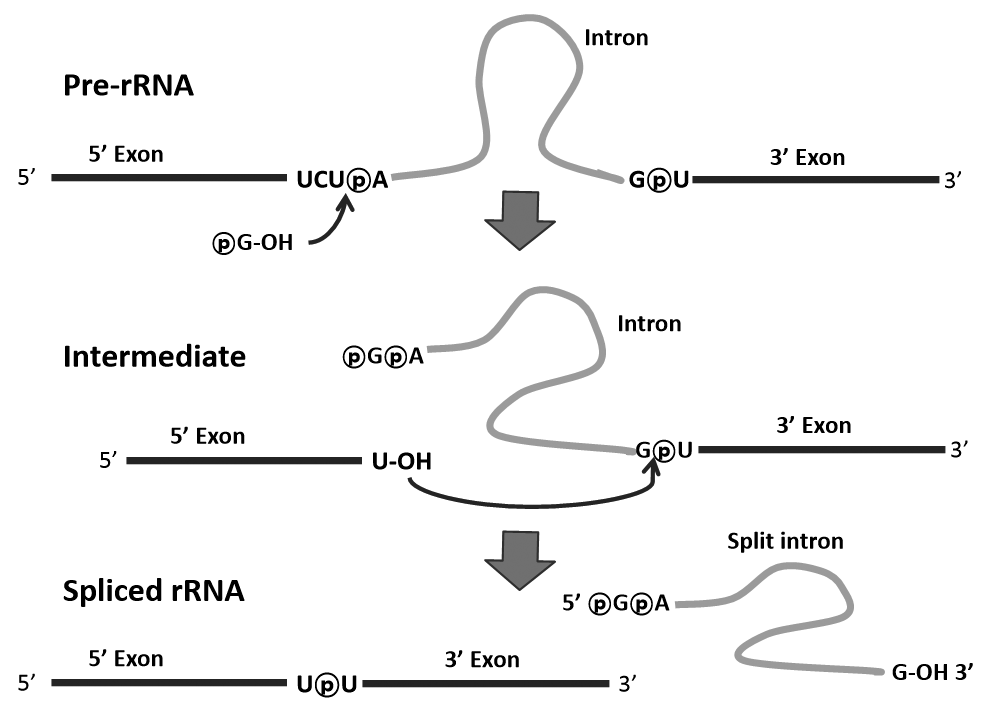
\includegraphics[width=\textwidth]{ART_Gim/fig.7_splicing_bw.png}%
 \end{center}%
 \caption{Cech's self-splicing mechanism
 %\label{ref:RNDiJ4MUJxdNH}(Zaug, Grabowski and Cech, 1983, p.582)
 \parencite[based on][p.582]{zaug_autocatalytic_1983}}\label{gim.fig7}
\end{figure}


Finally, I~would like to emphasize that whether an explanation is good or bad is not determined by any criteria but rather by its appropriateness or relevance to the topic determined in the given context. Ontic norms are instructions of mechanistic inquiries to discover patterns, not criteria to judge whether a~description is good. Ontic norms are self-contradictory because scientific achievements are thrown away as bad explanations. Completeness is an infeasible Utopian standard to be realized in science. It rather is realizable following the explainer's interests. A~philosophical distinction on explanatory normativity based on ontic norms seems a~pseudo-project.

Interestingly, Craver and Darden also agree on the pragmatic aspect of mechanistic explanation by acknowledging that ontic norms are compatible with agents' interests or given contexts by saying:

\myquote{
In speaking this way, we also intend to allow that a~schema can be complete and correct enough for the \textit{purposes} at hand without being fully complete or correct. One can acknowledge the ideals of completeness and correctness for descriptions of mechanisms while, at the same time, recognizing that science often traffics in \textit{idealized} and \textit{incomplete} schemas
%\label{ref:RNDBHgV0NHMyK}(Craver and Darden, 2013, p.9, emphasis added).
\parencite[][emphasis added]{craver_search_2013}.%
}
The pragmatic point of view was shown in the discussion of the conceptual dimension of the nature of explanation. Remind that the nature of mechanistic explanation is the tertiary relation among the representer, targets, and agent's goal in a~given context. When judging whether a~mechanistic explanation is successful, the explanation must be an adequate answer to a~question about why the explanandum phenomenon happens. According to van Fraassen
%\label{ref:RNDshKkR1q14q}(1980),
\parencite*[][]{van_fraassen_scientific_1980}, %
 an explanation is an answer to a~why-question. Here, I~do not apply van Fraassen's theory of explanation to mechanistic explanation. Still, I~emphasize that mechanistic explanations are evaluated by whether adequate representations explain the explanandum phenomenon under the agent's interest.

The same phenomenon can be explained differently depending on what aspects, to some degree, explain the phenomenon. For example, protein synthesis can be explained diversely concerning researchers' interests. Molecular biologists Watson and Crick were interested in the genetic flow from DNA to protein. The number of bases within nucleic acids is four, but the number of amino acids is twenty. So, the order of the bases in DNA determines what kinds of nucleic acids are in protein. By guessing the existence of a~single linear sequence of nucleic acids, or messenger RNA, they imagined how sequences of two or three bases correspond to 20 different types of amino acids. As a~result, the simple mechanism scheme, DNA$\to$RNA$\to$Protein, explains a~temporal order among essential entities within the mechanism. By contrast, biochemists Zamecnik and Hoagland focused on the energy flow in the form of ATP when amino acids are activated in synthesizing the peptide bond. Their chemical interest in protein synthesis led to the discovery of transfer RNA, which links the genetic code to amino acids. As a~result, Zamecnik's diagram in Fig. \ref{gim.fig1} explains how biomolecules interact with each other to synthesize the peptide bond.

Further, another biochemist, Cech, was interested in what enzymes mediate the splicing reactions of precursor ribosomal RNA before mRNA moves out of a~nucleus to synthesize protein. As a~result, Cech's diagram in Fig. \ref{gim.fig7} explains how splicing reactions, including cleavage of pre-rRNA, ligation, and cyclization, occur without enzymatic proteins. Besides them, numerous molecular biologists and biochemists have proposed models representing various aspects of the protein synthesis process, depending on their respective fields of interest. For the same protein synthesis process, molecular biologists focus on genetic information, and biochemists focus on energy equivalence. Even among the same biochemists, someone discovers the energy components needed for chemical reactions, and someone else discovers new functions of RNA. Likewise, the topic, scope, and purpose of explaining the protein synthesis process vary depending on the researcher's interests. The important thing is that all of them are significant achievements in biological sciences, even if each incompletely explains the full processes of protein synthesis. Whether a~mechanistic explanation is good or not depends upon the issue of \textit{how much an answer to the question is attained}.

As noted, Craver, Bechtel, and Wright adopt Salmon's distinction between ontic and epistemic. However, they disagree about the nature of mechanistic explanations. Craver
%\label{ref:RNDXpKAIeFKK5}(2006; 2007; 2014)
\parencites*[][]{craver_when_2006}[][]{craver_explaining_2007}[][]{kaiser_ontic_2014} %
 argues that the mechanistic explanation is also ontic, whereas Bechtel and Wright 
%\label{ref:RNDVFMWcu7K3P}(Wright and Bechtel, 2007; Wright, 2012; 2015)
\parencites[][]{wright_mechanisms_2007}[][]{wright_mechanistic_2012}[][]{wright_ontic_2015} %
 claim it is epistemic. Both agree that the mechanistic explanation should be based on something other than Hempel's account of scientific explanation. More precisely, they claim that a~mechanistic explanation does not include the laws of nature, and a~linguistic form of argument does not constrain the explanation units. Based on a~consensus of explanatory relevance in the first dimension, the three philosophers disagree on what mechanistic explanation is in the second dimension. Craver over-concentrates on the relational dimensions of mechanistic explanation in line with the first dimension of explanatoriness. On the contrary, Bechtel and Wright over-concentrate on the conceptual dimension of mechanistic explanation, such cognitive procedures independently from the first dimension. Remember that Craver rejects cognitive processes to identify causal factors of explanandum phenomena. As Illari mentions, Craver wants to proclaim an ontic constraint to examine mechanistic explanation in terms of mechanisms.

I~restate the first and second dimensions to show that the normative dimension can depend on the two dimensions. Ontic norms of mechanistic explanation originate from the first relational dimension on which all mechanists agree. Epistemic norms of mechanistic explanation stem from the second conceptual dimension of the nature of explanation. I~am emphasizing the non-existence of disagreement among ontic and epistemic theorists about a~claim that mechanistic explanation is an achievement from cognitive performances in practice. What is important is that epistemic norms are also instructions in mechanistic inquiries. This point has been similarly pointed out by many philosophers of science
%\label{ref:RNDq6KKYOeubQ}(Illari, 2013; van Eck, 2015; Sheredos, 2016; Kästner and Haueis, 2021).
\parencites[][]{illari_mechanistic_2013}[][]{van_eck_reconciling_2015}[][]{sheredos_re-reconciling_2016}[][]{kastner_discovering_2021}.%


Nonetheless, I~cannot entirely agree with the defenders of the epistemic priority of the mechanistic explanation as they maintain that there are separate epistemic constraints, such as generality or systematicity, which are either independent of or additional to the ontic constraint
%\label{ref:RNDh2G9YTeRNp}(van Eck, 2015; Sheredos, 2016).
\parencites[][]{van_eck_reconciling_2015}[][]{sheredos_re-reconciling_2016}. %
 The goal of understanding entities, activities, and their organizations is not independent of the ontic constraint, according to which we should discover the causal factors to explain a~phenomenon. Other epistemic norms for the mechanistic explanation may be helpful only after discovering all causal factors. Without the ontic constraint, any epistemic norms independently do not support the explanatory relevance of the mechanistic explanation. Discoveries, encompassing not only the components but also their organizational features within a~mechanism, serve as primary methodological guidance in biological sciences. Thus, ontic norms are not less worthy than any epistemic norms.

Are ontic and epistemic norms equally valuable? Illari
%\label{ref:RND9wQ7FGKuvY}(2013)
\parencite*[][]{illari_mechanistic_2013} %
 and Kastner \& Haueis 
%\label{ref:RNDcxC0bEqFNx}(2021)
\parencite*[][]{kastner_discovering_2021} %
 appear to answer this question affirmatively, a~stance with which I~concur. However, my focus extends beyond the relative significance of these norms. I~explored whether ontic norms warrant consideration in evaluating mechanistic explanations. I~demonstrated that ontic norms alone are insufficient for distinguishing between good and bad explanations. Consequently, both ontic and epistemic norms play essential roles, as neither norm conflicts independently of the demarcation problem concerning the quality of mechanistic explanations.

\section{Conclusion}
The paper analyzes ontic and epistemic debates in scientific explanation through the three-dimensional interpretation. Each debate dispute concerns a~particular issue: (1) explanatory formal framework, explanatory force, explanatory relevance between explanans and an explanandum; (2) nature of mechanistic explanation; and (3) normative constraints. This dimensional approach does not simply enumerate or give three names to different issues but is helpful to compare with participants' viewpoints in this debate. In addition, it provides a~practical framework to comprehend several philosophical perspectives in scientific explanation. Furthermore, those three dimensions have their philosophical issues but are also interconnected, so it can be helpful to clarify how to reconcile different normative constraints.

Recent ontic-epistemic debates are displayed among proponents of the New Mechanism. The mechanistic explanation is a~widespread explanatory practice in biological sciences. A~consensus exists that the explanatory relevance between the explanans and the explanandum is a~fundamental ontic constraint for a~mechanistic explanation. However, some philosophers have either focused on the epistemic nature of the mechanistic explanation or insisted on the epistemic norms or constraints over the ontic constraints. I~have shown that mechanistic explanations are better associated with the epistemic conception than with the ontic conception of explanation. I~emphasized the epistemic nature of mechanistic explanations by highlighting their strong dependence on the activities that represent the mechanism based on van Fraassen's pragmatic viewpoint. Contrary to stereotypical views held by New Mechanism advocates, I~proposed the linkage of mechanistic explanations to epistemic aspects such as logical validity, lawful grounds, and counterfactual inference. This is achieved by exploring the necessary conditions in linguistic representations of these mechanistic explanations. Further, I~addressed the philosophical issue of how mechanistic explanations should be evaluated.

Unlike many philosophers in the New Mechanism who stubbornly reject Hempel's model, I~suggested to view Hempel's conditions as necessary conditions for linguistic representation rather than sufficient conditions for scientific explanation. By noting that the usage of the ontic norms as criteria for distinguishing between good and bad explanations makes the mistake of dismissing many existing scientific achievements as ‘bad' explanations, I~assert the compatibility of mechanistic explanations with pragmatic aspects of explanation. Through this, I~carefully tried to reveal that the mechanistic explanation is significantly more related to the epistemic position than the ontic one.

\end{artengenv}
